%\documentclass[a4paper,10pt]{article}
\documentclass[a4paper]{article}
%\usepackage[paper=a4paper, hmargin=0.5cm, bottom=0.5cm, top=0.5cm]{geometry}
\usepackage[latin1]{inputenc}
\usepackage[T1]{fontenc}
\usepackage[spanish]{babel}
\usepackage{xspace}
\usepackage{xargs}
\usepackage{ifthen}
\usepackage{listings}
\usepackage{aed2-symb,aed2-itef,aed2-tad,caratula}
\usepackage{xcolor}
\usepackage{listings}
\usepackage{soul}
\usepackage{tikz}
\usepackage{MnSymbol}

%Tikz library
\usetikzlibrary{positioning}
\usetikzlibrary{arrows}
\usetikzlibrary{graphs,graphs.standard,quotes}
\usetikzlibrary[topaths]

\usepackage{graphicx}
\graphicspath{ {imagenes/} }
\usepackage{pgfplots}
\usepackage{tikz}

\usepackage[T1]{fontenc}
\usepackage{inconsolata}

\usepackage{color}

\definecolor{pblue}{rgb}{0.13,0.13,1}
\definecolor{pgreen}{rgb}{0,0.5,0}
\definecolor{pred}{rgb}{0.9,0,0}
\definecolor{pgrey}{rgb}{0.46,0.45,0.48}

\usepackage{listings}
\lstset{language=Java,
  showspaces=false,
  showtabs=false,
  breaklines=true,
  showstringspaces=false,
  breakatwhitespace=true,
  commentstyle=\color{pgreen},
  keywordstyle=\color{pblue},
  stringstyle=\color{pred},
  basicstyle=\ttfamily,
  moredelim=[il][\textcolor{pgrey}]{$$},
  moredelim=[is][\textcolor{pgrey}]{\%\%}{\%\%}
}

\usepackage[latin1]{inputenc} 
\usepackage{multirow}

\newcommand{\moduloNombre}[1]{\textbf{#1}}
\newcommand{\bigO}{\mathcal{O}}
\newcommand{\complejidad}[2]{\hfill $#1 \bigO(#2)$}

\let\NombreFuncion=\textsc
\let\TipoVariable=\texttt
\let\ModificadorArgumento=\textbf
\newcommand{\res}{$res$\xspace}
\newcommand{\tab}{\hspace*{7mm}}

\newcommandx{\TipoFuncion}[3]{%
\NombreFuncion{#1}(#2) \ifx#3\empty\else $\to$ \res\,: \TipoVariable{#3}\fi%
}
\newcommand{\In}[2]{\ModificadorArgumento{in} \ensuremath{#1}\,: \TipoVariable{#2}\xspace}
\newcommand{\Out}[2]{\ModificadorArgumento{out} \ensuremath{#1}\,: \TipoVariable{#2}\xspace}
\newcommand{\Inout}[2]{\ModificadorArgumento{in/out} \ensuremath{#1}\,: \TipoVariable{#2}\xspace}
\newcommand{\Aplicar}[2]{\NombreFuncion{#1}(#2)}

\newlength{\IntFuncionLengthA}
\newlength{\IntFuncionLengthB}
\newlength{\IntFuncionLengthC}
%InterfazFuncion(nombre, argumentos, valor retorno, precondicion, postcondicion, complejidad, descripcion, aliasing)
\newcommandx{\InterfazFuncion}[9][4=true,6,7,8,9]{%
  \hangindent=\parindent
  \TipoFuncion{#1}{#2}{#3}\\%
  \textbf{Pre} $\equiv$ \{#4\}\\%
  \textbf{Post} $\equiv$ \{#5\}%
  \ifx#6\empty\else\\\textbf{Complejidad:} #6\fi%
  \ifx#7\empty\else\\\textbf{Descripci\'on:} #7\fi%
  \ifx#8\empty\else\\\textbf{Aliasing:} #8\fi%
  \ifx#9\empty\else\\\textbf{Requiere:} #9\fi%
}

\newenvironment{Interfaz}{%
  \parskip=2ex%
  \noindent\textbf{\Large Interfaz}%
  \par%
}{}

\newenvironment{Representacion}{%
  \vspace*{2ex}%
  \noindent\textbf{\Large Representaci\'on}%
  \vspace*{2ex}%
}{}

\newenvironment{Algoritmos}{%
  \vspace*{2ex}%
  \noindent\textbf{\Large Algoritmos}%
  \vspace*{2ex}%
}{}


\newcommand{\titlex}[1]{
  \vspace*{1ex}\par\noindent\textbf{\large #1}\par
}

\newenvironmentx{Estructura}[2][2={estr}]{%
  \par\vspace*{2ex}%
  \TipoVariable{#1} \textbf{se representa con} \TipoVariable{#2}%
  \par\vspace*{1ex}%
}{%
  \par\vspace*{2ex}%
}%

\newboolean{EstructuraHayItems}
\newlength{\lenTupla}
\newenvironmentx{Tupla}[1][1={estr}]{%
    \settowidth{\lenTupla}{\hspace*{3mm}donde \TipoVariable{#1} es \TipoVariable{tupla}$($}%
    \addtolength{\lenTupla}{\parindent}%
    \hspace*{3mm}donde \TipoVariable{#1} es \TipoVariable{tupla}$($%
    \begin{minipage}[t]{\linewidth-\lenTupla}%
    \setboolean{EstructuraHayItems}{false}%
}{%
    $)$%
    \end{minipage}
}

\newcommandx{\tupItem}[3][1={\ }]{%
    %\hspace*{3mm}%
    \ifthenelse{\boolean{EstructuraHayItems}}{%
        ,#1%
    }{}%
    \emph{#2}: \TipoVariable{#3}%
    \setboolean{EstructuraHayItems}{true}%
}

\newcommandx{\RepFc}[3][1={estr},2={e}]{%
  \tadOperacion{Rep}{#1}{bool}{}%
  \tadAxioma{Rep($#2$)}{#3}%
}%

\newcommandx{\Rep}[3][1={estr},2={e}]{%
  \tadOperacion{Rep}{#1}{bool}{}%
  \tadAxioma{Rep($#2$)}{true \ssi #3}%
}%

\newcommandx{\Abs}[5][1={estr},3={e}]{%
  \tadOperacion{Abs}{#1/#3}{#2}{Rep($#3$)}%
  \settominwidth{\hangindent}{Abs($#3$) \igobs #4: #2 $\mid$ }%
  \addtolength{\hangindent}{\parindent}%
  Abs($#3$) \igobs #4: #2 $\mid$ #5%
}%

\newcommandx{\AbsFc}[4][1={estr},3={e}]{%
  \tadOperacion{Abs}{#1/#3}{#2}{Rep($#3$)}%
  \tadAxioma{Abs($#3$)}{#4}%
}%

\usepackage{pdfpages}
% \lstset {
%     language=C++,
%     backgroundcolor=\color{black!5}, % set backgroundcolor
%     basicstyle=\footnotesize,% basic font setting
% }

\usepackage{xcolor,colortbl}
\definecolor{green}{rgb}{0.1,0.1,0.1}
% Enter this in the cell you wish to color a light grey.
% NB: the word 'gray' here denotes the grayscale color scheme, not the color grey. '0.9' denotes how dark the grey is.

\definecolor{pblue}{rgb}{0.13,0.13,1}
\definecolor{pgreen}{rgb}{0,0.5,0}
\definecolor{pred}{rgb}{0.9,0,0}
\definecolor{pgrey}{rgb}{0.46,0.45,0.48}

\usepackage{listings}
\lstset{language=Java,
  showspaces=false,
  showtabs=false,
  breaklines=true,
  showstringspaces=false,
  breakatwhitespace=true,
  commentstyle=\color{pgreen},
  keywordstyle=\color{pblue},
  stringstyle=\color{pred},
  basicstyle=\ttfamily,
  moredelim=[il][\textcolor{pgrey}]{$$},
  moredelim=[is][\textcolor{pgrey}]{\%\%}{\%\%}
}

\begin{document}

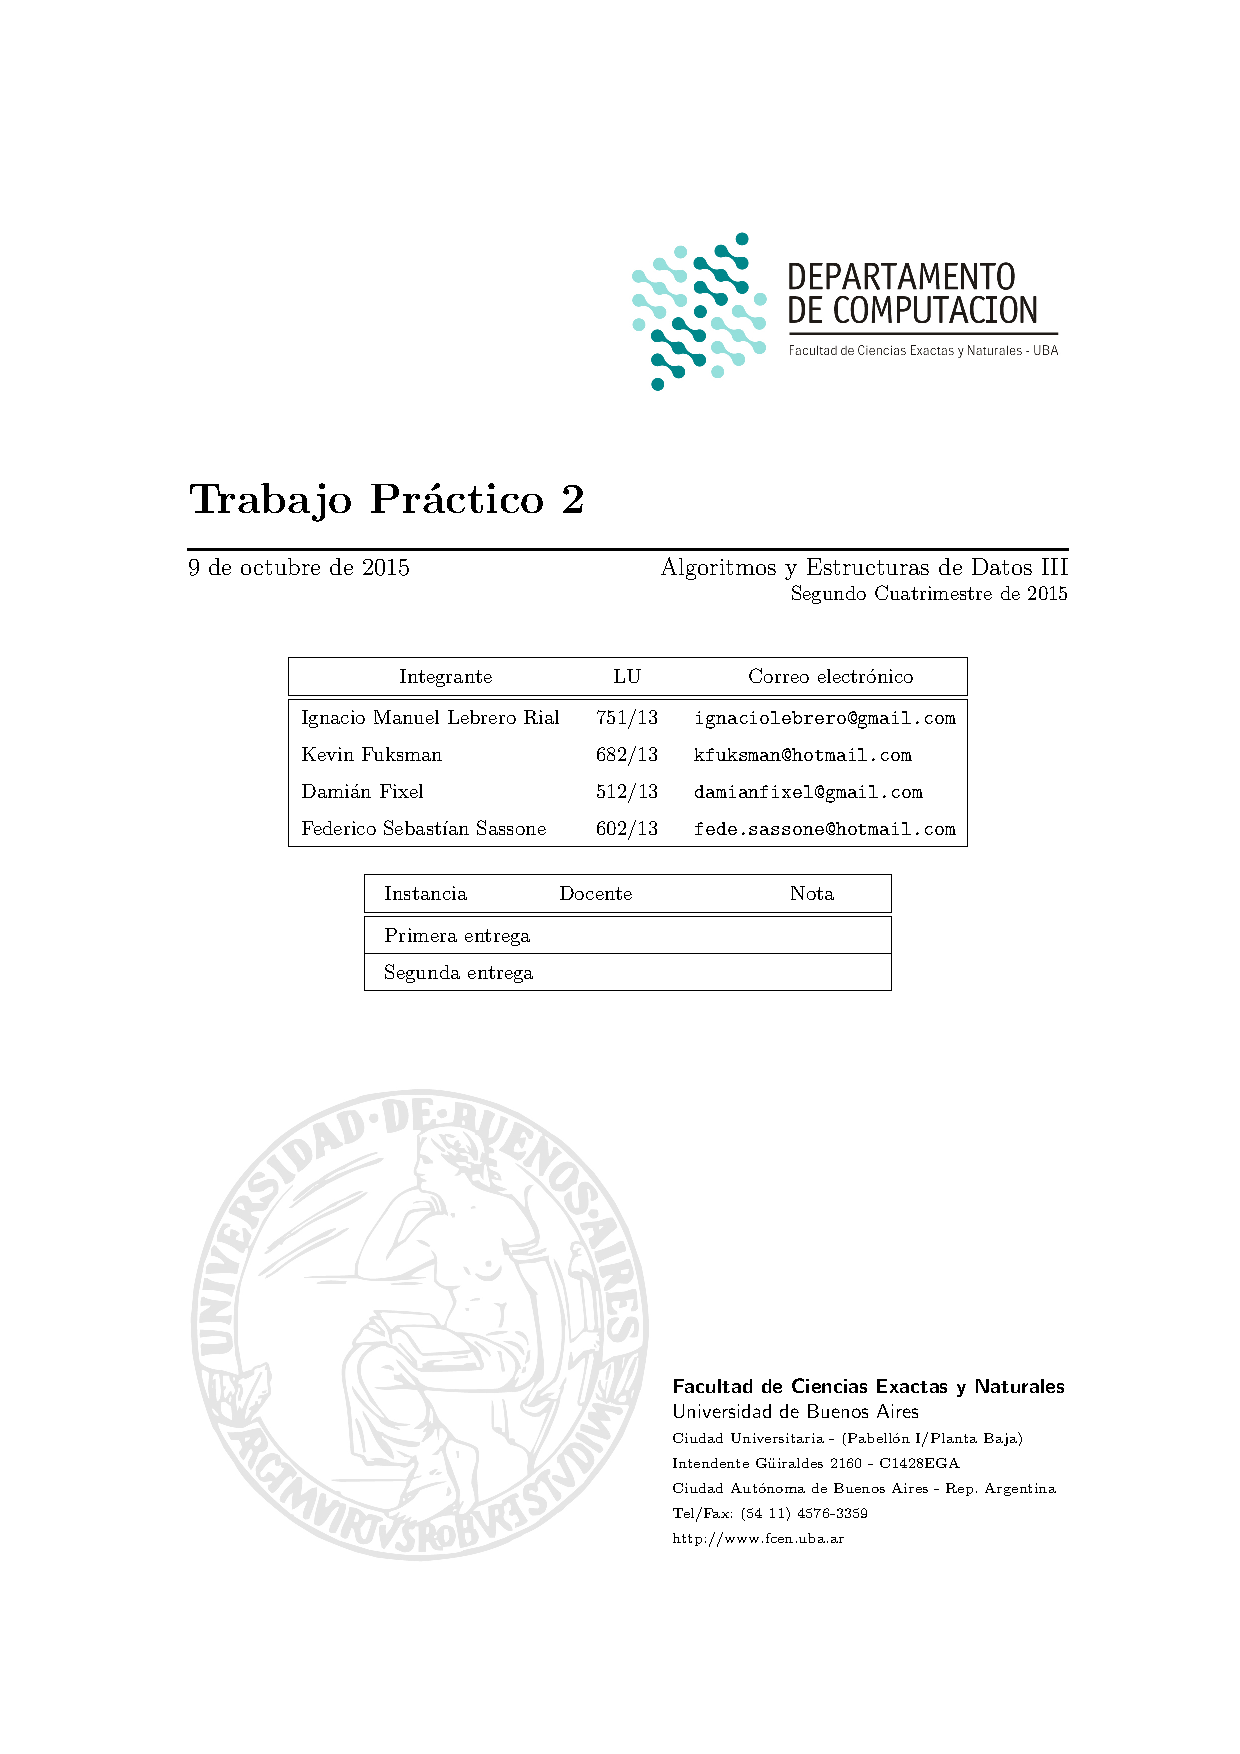
\includepdf{caratula}

% compilar 2 veces para actualizar las referencias
\tableofcontents

\pagebreak
\section{Ejercicio 1}
\subsection{Problema: Saliendo del freezer}

Estamos en el a\~no 2048 y el Pabell\'on 0+infinito es todo un \'exito. Los alumnos de Algoritmos III est\'an
contentos porque van a cursar este cuatrimestre en un aula que est\'a en el piso N, que es el m\'as alto de
todos. Con los avances de la ciencia y la tecnolog\'ia, escaleras y ascensores han quedado obsoletos, y la
forma de subir de un piso a otro es a trav\'es de portales. El nuevo pabell\'on tiene P portales, cada uno
de los cuales permite subir de un piso A a un piso m\'as alto B (para bajar de piso hay que tirarse con
paraca\'idas al piso 0 y luego volver a subir de ser necesario). Uno de los alumnos, que estaba cursando en
el segundo cuatrimestre de 2015 y fue congelado por el m\'etodo de criogenia, acaba de ser descongelado
y no puede creer lo buenos que est\'an estos portales, algo que en su \'epoca no exist\'ia. Luego de completar
todos los censos de estudiantes desde el a\~no 2016 en adelante, este alumno quiere usar la mayor cantidad
de portales posibles para llegar al piso N y as\'i seguir cursando Algoritmos III. Dise\~nar un algoritmo de complejidad $\bigO(N^2)$ para calcular la mayor cantidad de portales que puede utilizar el alumno para subir desde planta baja al piso N (sin tirarse nunca con paraca\'idas). Se asegura que en toda instancia del problema es posible realizar el recorrido deseado, y que no hay m\'as de un portal que comunique el mismo
par de pisos. 



\subsubsection{Explicacion del Problema}
Para este problema se cuenta con un grafo dirigido, donde cada vertice pertenece a un piso y sus ejes conectan con vertices pertenecientes al mismo piso, en cuyo caso seran bidireccionales o unidireccionales en caso contrario.

%dibujo de muestra

El objetivo sera, dadas las conexiones de vertices de distintos pisos entre si, como moverse desde el vertice ubicado en el metro 0 del piso 0 hasta algun vertice en el piso N, de manera que utilice la mayor cantidad de vertices posibles. 

%dibujo de ejemplo

Observar que como los vertices de distintos pisos estan conectados de manera unidireccional, no se generaran ciclos dentro del grafo.

\subsubsection{Explicacion del Desarrollo}
Para conseguir la cantidad maxima de portales que se pueden utilizar para ir desde el piso 0 hasta el ultimo desarrollaremos un algoritmo basado em programacion dinamica. Dentro de una matriz, las filas tendran el inicio del portal y las columnas tendran el destino. La parte inferior de la diagonal no se calculara porque no podemos dirigirnos hacia abajo.\\
Luego se inicializara la matriz completa en -2, a exepcion de la diagonal que tendra 0 (ya que la cantidad de portales para moverse entre el mismo piso es 0). Una vez iniciada la matriz llamada M, para un portal P que comunica los pisos p1 y p2, pondremos en $M[p1,p2]$ el valor -1. Quedando la matriz conformada de la siguiente manera:
\subitem
Las celadas inferiores a la diagonal, no interesan.
\subitem
Las celdas en la diagonal, tienen valor 0
\subitem
Las celdas superiores a la diagonal tienen valor -2 a menos que exista un portal que conecte esos pisos. En ese caso el valor es -1 \\

Luego de armar la matriz: \\
1)Para cada piso $i$ se pregunta si se conecta con el ultimo. En caso afirmativo se llena el vector $mejores[i]$ con 1. Caso contrario con -2.\\

2) se recorre la matriz de abajo hacia arriba y de derecha a izquierda y se completa de la siguiente manera: \\

Sean i,j los indices de la actual iteracion, si existe un portal desde el piso i al piso j y ademas el piso j esta conectado al ultimo piso, entonces encontramos una posible forma de ir desde el piso i hasta el ultimo: trasladarse del i al j, y luego el camino correspondiente entre j y el ultimo. Tambien sabemos que la longitud del camino correspondiente de ir del piso i al ultimo piso es igual a la longitud de ir de j al ultimo piso, mas 1 (el portal que nos lleva de i a j).\\
Sin embargo no podemos asegurarnos que este sea el mejor camino, por lo que luego de realizar esta operacion, diremos que $mejores[i]$ es el maximo entre el valor que ya tenia (que era el maximo hasta el momento) y el nuevo valor descubierto. 

\subsection{Justificaci\'on y Complejidad}
\begin{lstlisting}
FOR i desde 0 hasta matriz.length       // O(N)
    FOR j desde 0 hasta matriz.length   // O(N)
        IF j == i THEN                  // O(1)
            matriz[i][j] = 0            // O(1)
        ELSE            
            matriz[i][j] = -2           // O(1)
        ENDIF
    ENDFOR
ENDFOR
\end{lstlisting}


Costo final de inicializacion de estructuras : $\bigO(n^2)$.

\begin{lstlisting}
FOREACH portales as portal           // O(cantidadPortales)
    matriz[portal.getFrom()][portal.getTo()] = -1  
    //seteo un -1 en las celdas de la matriz que correspondan a pisos conectados O(1)
ENDFOREACH
\end{lstlisting}


%Esta funci\'on se puede sumar al costo de la inicializacion de las estructuras o bien podriamos acotarlo por $\bigO(n^2)$.


El costo de la funci\'on anterior esta determinada por la cantidad de portales que haya en el edificio. La cantidad m\'axima de portales posibles es ex\'actamente la cantidad de aristas del grafo completo:\\
Habiendo $n$ pisos ($n$ nodos),  $\frac{n*(n-1)}{2}$. \\
Luego, el costo de esta secci\'on es de $\bigO(\frac{n-1}{2} * n)$ = $\bigO(n)$.

%Si analizamos los portales como aristas en un grafo, y como podemos afirmar, un grafo completo tiene V*(V-1) /2, siendo V la cantidad de vertices. Podemos acotar la cantidad de portales por $N^2$ para luego poder determinar que el costo de esta seccion es de  $\bigO(n^2)$.
%Aca se podria ser mas especifico con la cota de portales, porque por enunciado no existe un portal desde un piso superior hacia uno inferior, reduciendo la cota de N^2.
\pagebreak


\begin{lstlisting}
FOR i desde 0 hasta matriz.length -1                // O(N) 
    IF matriz[i][matriz.length -1] == -1   THEN     // O(1)
        matriz[i][matriz.length-1] = 1              // O(1)
        mejores[i] = 1                              // O(1)
    ELSE 
	mejores[i] = -2                             // O(1)
    ENDIF
ENDFOR
//Ponemos 1 en [i][piso n] si el piso i se conectaba con el ultimo piso, para todo i.
\end{lstlisting}



Costo de esta secci\'on : $\bigO(N)$

\begin{lstlisting}
FOR i desde matriz.length -2 hasta 0                        //  O(N)
    FOR j desde matriz.length -2 hasta i                    //  O(N)
        IF matriz[i][j] == -1 && mejores[j] > 0   THEN      //  O(1)
            matriz[i][j] = mejores[j] + 1                   //  O(1)
            mejores[i] = Maximo(mejores[i], matriz[i][j])   //  O(1)
        ENDIF
    ENDFOR
ENDFOR
    RETURN mejores[0]     // O(1)
    // Si hay conexion en [i][j] y j se conectaba con el ultimo piso, la celda [i][j] vale lo que valia el vector[j]. Por como recorremos la matriz, vamos guardando los "portales maximos" en cada iteracion
\end{lstlisting}
Costo de esta secci\'on : $\bigO(N^2)$

Si sumamos todas las secciones de nuestro algoritmo es facil notar que la complejidad es $\bigO(2 * n^2 + n)$, la cual podemos acotarla por $\bigO(n^2)$ que era la complejidad pedida.

\pagebreak
\subsection{Correctitud}     

Vemamos como se comporta, una vez inicializada la estructura, nuestra funci\'on recursiva $F$; que asigna valores a las celdas de la matriz para resolver el problema.\\

F(i , j) = \left \{ \begin{matrix} 1  & \mbox{si}\mbox{ j == n \&\& matriz[i][j] == 1}\\
-2  & \mbox{si }\mbox{ j == n \&\& matriz[i][j] != 1}
\\ \smash{\displaystyle\max_{0 \leq k \leq n}} F(i,k) + H& \mbox{si }n\mbox{ j != n}\end{matrix}\right.\\ \\ \\ 


Nuevamente, como aclaramos en la secci\'on complejidad, nuestra recursi\'on hace lo siguiente:
Verifica conexiones de los pisos i con el \'ultimo piso, si las hay, escribe 1 en [i][piso n] (pues 1 es el maximo de portales en llegar de i al \'ultimo.).\\
Si no hay conexi\'on, coloca un -2 pues vamos a ignorar esa celda.\\

Luego, desde abajo a la derecha hacia la izquierda y arriba, chequea si los pisos i se conectan con j. Si lo hacen y a su vez j se conecta con el piso n, toma el m\'aximo entre  mejores[i] y mejores[j+1].\\

Esto chequea, para cada piso, cu\'antos portales tarda en llegar hasta el \'ultimo, y si hay forma de llegar pasando por los pisos superiores (que ya recorrimos).\\ 
La comparaci\on entre mejores[i] y mejores[j+1] es porque comparamos el m\'aximo valor desde el piso i hasta n contra el m\'aximo valor en el piso j + la conexion de i con j.\\

En cada iteraci\'on vamos a conseguir la cantidad m\'axima de portales para llegar desde el piso i hasta el n. Comenzamos con i en el ante\'ultimo piso y vamos bajando; esto nos garantiza que al final del recorrido vamos a estar en el piso 0, por ende tendremos la cantidad m\'axima de portales necesaria para llegar desde el piso 0 hasta el n, que es lo que busc\'abamos.\\

En la funci\'on, la variable H va a estar dada por el resultado de la funci\'on iterativa max. Si el resultado es -2(es decir, no hay max pues no hay conexion de i con k) entonces H es 0, caso contrario es 1 (incrementamos en 1 al maximo que es distinto a -2, pues le agregamos al maximo que habiamos encontrado una conexion extra de i a k).\\

Una vez entendida nuestra funci\'on recursiva veamos gr\'aficamente c\'omo funciona tomando la siguiente matriz: 
\pagebreak

\begin{center}
  \begin{tabular}{| l | l | c | r | r | r | r |}
    \hline
   & \multicolumn{6}{|c|}{Portal} \\ \hline
    & Al 0 & Al 1 & Al 2 & Al 3 & Al 4 & Al 5 \\ \hline
    
    Piso 0 &\cellcolor{red} & $\leftarrow$ & $\leftarrow$  & $\leftarrow$ & $\leftarrow$  & $\leftarrow$ \\ \hline
    Piso 1 &\cellcolor{red} & \cellcolor{red} & $\leftarrow$  & $\leftarrow$ & $\leftarrow$  & $\leftarrow$ \\ \hline
    Piso 2 &\cellcolor{red} & \cellcolor{red} & \cellcolor{red} & $\leftarrow$ & $\leftarrow$  & $\leftarrow$ \\ \hline
    Piso 3 &   \cellcolor{red} & \cellcolor{red} & \cellcolor{red} & \cellcolor{red} & $\leftarrow$ & $\leftarrow$  \\ \hline
    Piso 4 &   \cellcolor{red} & \cellcolor{red} & \cellcolor{red} & \cellcolor{red} & \cellcolor{red} & $\leftarrow$  \\ \hline
    Piso 5 &\cellcolor{red} & \cellcolor{red} & \cellcolor{red} & \cellcolor{red} &\cellcolor{red}  &\cellcolor{red}  \\ \hline
    
  \end{tabular}
\end{center}


Las celdas de color rojo no son recorridas por nuestro algoritmo ya que no hay portales que vayan a un piso inferior o al mismo piso. S\'olo recorremos las que tienen flechas hacia la izquierda.\\

Una vez iniciada la matriz, tendr\'an -1 las celdas que representen una conexi\'on entre pisos. Ejemplo, si hay un -1 en [Piso 3][Al 4] significa que hay un portal del piso 3 al 4. Si hay un -2 en esta misma celda, significar\'a que estos pisos no est\'an conectados.\\

Ahora recorremos la columna de Al5 reemplazando los -1 con 1. Esto deja moment\'aneamente un 1 como cantidad m\'axima de portales desde los pisos correspondientes hasta el piso n. Adem\'as guardamos en mejores[i] ese valor. Ejemplo, [Piso 3][Al 5] era -1, lo cambiamos a 1 y mejores[3] ahora es 5. Caso contrario quedan en -2 ambos, celda de la matriz e \'indice del vector. \\

Luego recorremos el resto de la matriz;\\comenzando desde $"$abajo a la derecha$"$, [Piso3][Al4], verificamos si hay conexi\'on. Si no la hay, no hacemos nada y nos movemos a la izquierda, de no tener una celda con flecha como es el caso, vamos hacia arriba, [Piso2][Al4]. Esto mantiene nuestro "invariante" de la estructura, con el que garantizamos que siempre tenemos el m\'aximo hasta el lugar recorrido, ya que el que no haya conexi\'on significa que es una celda que no nos interesa.\\

Ahora, si hay conexi\'on en [Piso3][Al4] y adem\'as mejores[4] es mayor a 0 (condici\'on importante porque significa que hay forma de llegar desde 4 a 5, caso contrario no nos interesa la conexi\'on [Piso3][Al4]), lo que hacemos es tomar [Piso3][Al4] y asignarle Mejores[4] + 1 (ya que la cantidad de portales para ir del 3 al 5 es igual a la catidad de portales para ir del 4 al 5 mas el portal que nos lleva del 3 al 4) , y luego a mejores[3] el m\'aximo entre el valor viejo de mejores[3] y el nuevo valor de [Piso3][Al4].\\

En este paso tomamos una celda que conectaba a un piso i con uno j y le asignamos la m\'axima cantidad de portales para llegar al \'ultimo piso si era posible, guardando adem\'as en mejores[i] esa m\'axima cantidad.\\
Una vez realizado esto, nos seguimos moviendo por la matriz.
Como empezamos desde el \'ultimo piso y vamos bajando, garantizando que en cada iteraci\'on guardamos el m\'aximo posible en las celdas y en mejores[i] para todo piso i.\\

Entonces, finalmente, cuando terminamos de recorrer el Piso0 tendremos en mejores[0] la cantidad m\'axima de portales.\\

Como no asumimos nada de la matriz antes de aplicarle el algoritmo y analizamos todos los posibles $"$If's$"$, esta correctitud vale para toda matriz.



\subsection{Tests}

Asumimos que no habr\'ia mejores y peores casos, ya que no importa c\'omo se distribuyan los portales, si o si nuestro algoritmo recorr\'ia toda la matriz (la diagonal superior). 

Como no utilizamos ning\'un tipo de poda, (como por ejemplo no chequear los pisos que no se conectan con los siguientes) en los tests se ver\'a reflejado que no existe ning\'un mejor ni peor caso. Esto sucede por un motivo en particular: si bien la parte inferior de la matriz no la tocamos en ningun momento, sin importar el caso en el que estemos, siempre vamos a estar completando y revisando toda la matriz del lado superior, por ende la unica diferencia que hay entre dos casos cualquiera es el resultado de la operaci\'on elemental y no la cantidad que estemos haciendo; es por eso que aunque llenemos nuestra matriz con portales o la dejemos vac\'ia, el tiempo de computo no se ver\'a dr\'asticamente afectado.

\subsubsection{Performance}
A la hora de hacer nuestras mediciones, cre\'iamos que si bien nuestra func\'ion tiene una complejidad de $\bigO(n^2)$, en realidad iba a ser mucho menor ya que las operaciones que realiz\'abamos eran sobre la mitad de la matriz.\\




\begin{figure}[h!]
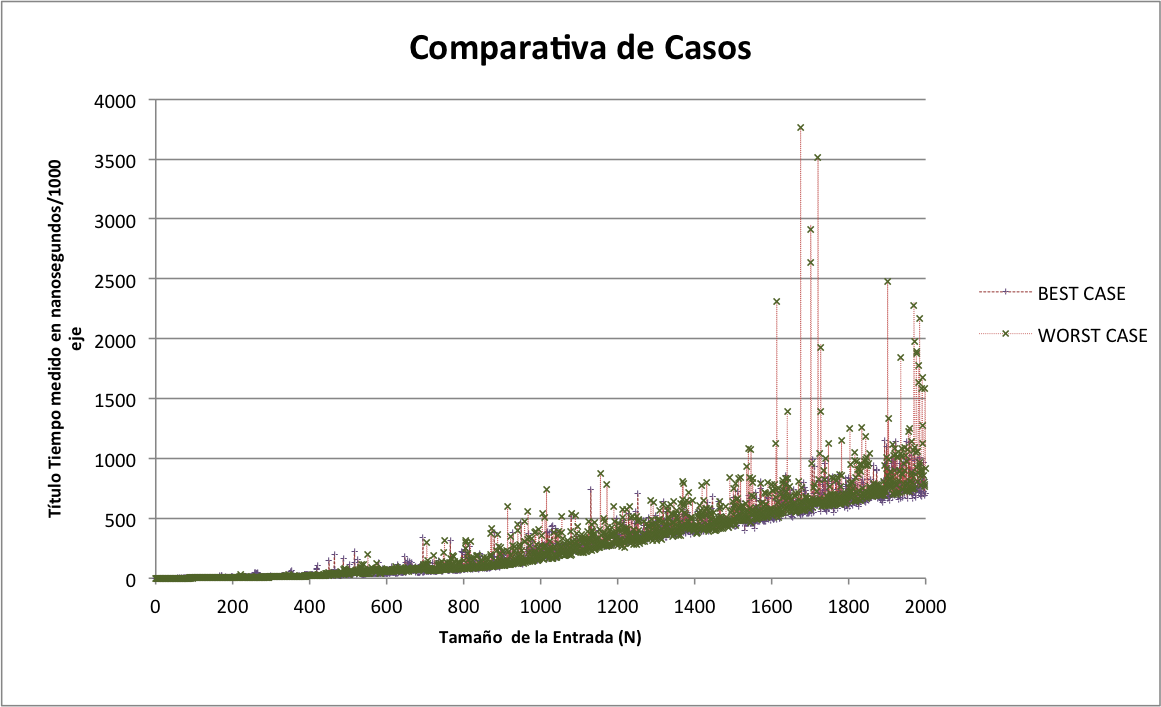
\includegraphics[width=140mm]{ej1-comp-tp2.png}
\centering
\caption{Comparaci\'on de matrices sin portales y completas.}
\label{overflow3}
\end{figure}

Efectivamente sucede lo que sospechabamos en la seccion anterior: En la primera figura vemos como el mejor y el peor caso se comportan asintoticamente de la misma manera ya que no importa qu\'e portales tengamos, la parte superior de la matriz se completa siempre.\\ 

\begin{figure}[h!]
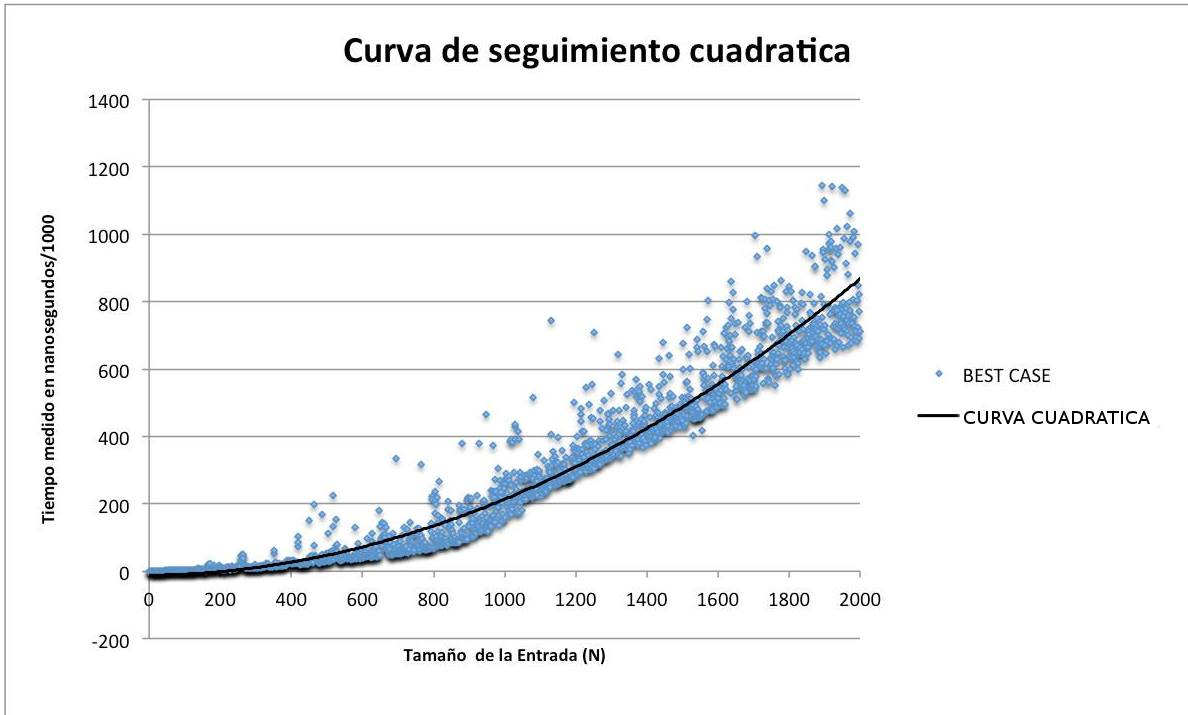
\includegraphics[width=140mm]{ej1-comp2-tp2.png}
\centering
\caption{Comparaci\'on de matrices sin portales y funcion cuadratica.}
\label{overflow3}
\end{figure}

En este segundo gr\'afico podemos ver que el comportamiento del algoritmo se puede aproximar con una curva cuadr\'atica multiplicada por una constante baja. Esto sucede porque como hab\'iamos mencionado anteriormente, nunca se recorre la matriz entera.

\pagebreak

\pagebreak

\section{Ejercicio 2}

\subsection{Problema: Algo Rush}
El Pabell\'on 0+infinito acaba de reabrir sus puertas con la novedad de que ahora tiene P portales que
son bidireccionales; asimismo, los paraca\'idas fueron eliminados por considerarse inseguros. Cada piso del renovado pabell\'on consta de un pasillo de L metros de longitud, y cada portal permite viajar entre
posiciones espec\'ficas de los pasillos de dos pisos. M\'as concretamente, cada portal puede describirse por
medio de cuatro enteros no negativos A, DA, B y DB, los cuales indican que el portal comunica el
piso A, a DA metros del comienzo del pasillo de ese piso, con el piso B, a DB metros del comienzo
del pasillo de ese piso. Los alumnos, acostrumbrados a los portales que s\'olo permitan subir, est\'an un
poco confundidos al poder utilizar un mismo portal tanto para subir como para bajar entre dos pisos, o
incluso para moverse entre posiciones diferentes dentro del pasillo de un mismo piso. Todos los alumnos
de Algoritmos III quieren llegar primero a la clase, que es en un aula que est\'a al final del piso N (el m\'as
alto del pabell\'on). Dise\~nar un algoritmo de complejidad O(NL + P) para calcular la m\'inima cantidad
de segundos que se necesitan para llegar del comienzo del pasillo del piso 0 al final del pasillo del piso
N, suponiendo que recorrer un metro requiere 1 segundo, y utilizar cualquier portal requiere 2 segundos
(en cualquiera de las dos direcciones posibles). Se asegura que en toda instancia del problema es posible
realizar el recorrido deseado, y que no hay m\'as de un portal que comunique las mismas posiciones del
mismo par de pisos. No obstante, puede haber m\'as de un portal que comunique el mismo par de pisos,
y portales que comuniquen posiciones diferentes dentro del pasillo de un mismo piso.\\

Este problema esta planeado de una manera parecida al anterior tendiendo como diferencia principal que ahora los portales son bidireccionales y que el primero quiere maximizar la cantidad de portales usados y este desea minimizar el tiempo para llegar desde el principio hasta el final. La medida del tiempo, com bien dice el enunciado, depende de la cantidad de portales que utilicemos y de la cantidad de metros que caminemos. Cada portal que utilicemos nos tomara 2 segundos y cada metro que camienmos nos aumentara 1 segundo.

\pagebreak
\subsubsection{Explicacion del Problema}
    El problema consiste en minimizar la cantidad de tiempo que se tarda en llegar desde el inicio de la planta baja hasta el final del ultimo piso. Esto puede ser representado por un grafo donde los nodos representan los portales (el inicio de la planata baja y el final del ultimo piso tambien) y los ejes los metros (o segundos) entre un portal y otro, observar que para este caso los ejes son bidireccionales ya que se puede ir y volver por los portales. Si el eje representa la conexion entre dos portales que esten conectados su peso sera 2 y, de no estar conectados y ser adyacentes en el mismo piso, equivaldra a la distancia que exista entre ambos.
    
    \begin{figure}
    \centering
    
    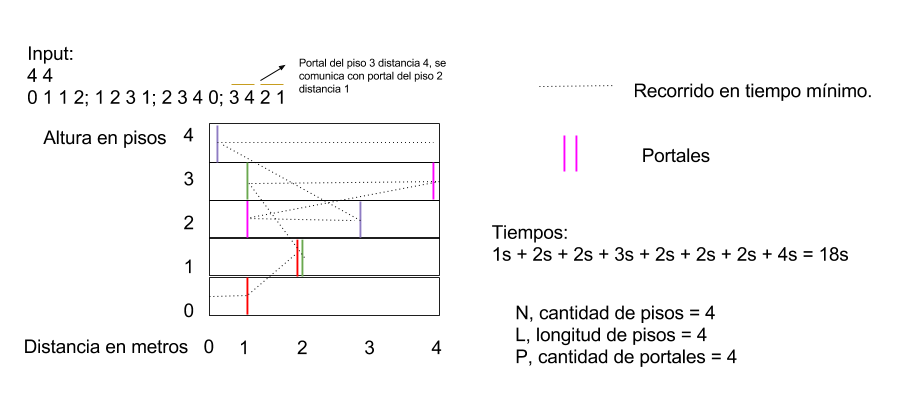
\includegraphics[scale=0.5]{imagenes/dibujito2.png}
    \caption{representacion de pisos y portales y su solucion}
    \label{fig:my_label}
    
    \tikzset{main node/.style={circle,fill=white!20,draw,minimum size=0.5cm,inner sep=0pt},}
\begin{tikzpicture}
    %\begin{scope}[xshift=4cm]
    \node[main node] (1) {1};
    \node[main node] (2) [right = 0.7cm  of 1] {2};
    \node[main node] (3) [above right = 0.7cm and 0.5cm of 2] {3};
    \node[main node] (4) [right = 0.1cm of 3] {4};
    \node[main node] (5) [above left = 0.7cm and 0.5cm of 3] {5};
    \node[main node] (6) [right = 1.5cm of 5] {6};
    \node[main node] (7) [above = 0.7cm of 5] {7};
    \node[main node] (8) [right = 2cm of 7] {8};
    \node[main node] (9) [above left = 0.7cm and 0.5 of 7]{9};
    \node[main node] (10) [right = 3.0cm of 9] {10};


    \path[draw,thick]
    (1) edge node {$1$} (2)
    (2) edge node {$2$} (3)
    (4) edge node {$2$} (7)
    (6) edge node {$2$} (9)
    (8) edge node {$2$} (5)
    (2) edge node {$2$} (3)
    (3) edge node {$0$} (4)
    (5) edge node {$2$} (6)
    (7) edge node {$3$} (8)
    (9) edge node {$4$} (10)
    ;
    %\end{scope}
\end{tikzpicture}

    \caption{representacion en un grafo del ejemplo anterior}
    \end{figure}
    
    Para solucionar el problema se cuenta con una cota m\'axima de $O(N*L + P)$ con N cantidad de pisos, L longitud de cada piso y P cantidad total de portales.
    
\subsubsection{Explicacion del Desarrollo}
    Se cuenta con un grafo con pesos distintos en sus ejes, sobre el mismo habra una cantidad total de $P + 2$ nodos (cantidad de portales mas nodo inicial y final). 
    A continuacion se analizara una modificacion del grafo, para esto definimos: \\

    Sea $G$ un grafo conexo con pesos posisitivos en sus ejes y $v$,$w$ cualquier par de vertices adyacentes de $G$, llamamos $G'$ al grafo donde el peso $p$ en el eje que conecta v con w es reemplazado por $p - 1$ nodos intermedios (de peso 1 en sus ejes) entre v y w, siendo asi $G'$ un grafo con peso uniforme en sus ejes. \\

    \begin{center}
        \tikzset{main node/.style={circle,fill=white!20,draw,minimum size=1cm,inner sep=0pt},}
\begin{tikzpicture}
    \node[main node] (1) {$A$};
    \node[main node] (2) [right = 1.5cm of 1]  {$B$};

    \path[draw,thick]
    (1) edge node {$2$} (2)
    ;
    %%
    \begin{scope}[xshift=4cm]
    \node[main node] (1) {$A$};
    \node[main node] (3) [right = 1.5cm  of 1] {};
    \node[main node] (2) [right = 1.5cm  of 3] {$B$};

    \path[draw,thick]
    (1) edge node {$1$} (3)
    (3) edge node {$1$} (2)
    ;
    \end{scope}
\end{tikzpicture}
\\Ejemplo nodos fantasma para un eje de peso 2
    \end{center}
    
    El nuevo grafo $G'$ colocara nodos intermedios entre los nodos de $G$, como puede haber un nodo en cada punta de los pisos (metro 0 y L) se pueden generar hasta $L-2$ nodos intermedios por piso, aplicandolo a todos los pisos queda $N * (L - 2)$ nodos totales, falta tener en cuenta las conexiones entre portales a las cuales se les agrega un nodo a cada una con lo que quedaria $N * (L - 2) + P$ con lo que puede ser acotado por $N*L + P$ nodos totales \endl\\
    
    Por lo visto en clase el algoritmo $BSF$ tiene complejidad lineal sobre la cantidad de nodos del grafo y puede encontrar el camino minimo entre $2$ nodos si los pesos son constantes en sus ejes, si trabajamos con $G'$ podemos ver que cumple con las condiciones que pide BFS y su complejidad sera $O($cantidad de nodos de $G') = O(N*L + P)$ que es la complejidad pedida.
    
    \begin{figure}
    \centering
    \tikzset{main node/.style={circle,fill=white!20,draw,minimum size=0.75cm,inner sep=0pt},}
\begin{tikzpicture}
    
        \node[main node] (1) {0};
        \node[main node] (2) [right = 3.5cm of 1]  {};
        \node[main node] (3) [above = 1.5cm of 1]  {};
        \node[main node] (4) [right = 1.9cm of 3]  {};
        
        \node[main node] (5) [above = 3.5cm of 2]  {};
        \node[main node] (6) [left  = 1.8cm of 5]  {};
    
        \path[draw,thick]
        (1) edge node {} (2)
        (2) edge node {} (3)
        (2) edge node {} (5)
        (3) edge node {} (4)
        (3) edge node {} (6)
        (4) edge node {} (6)
        (5) edge node {} (6)
        (5) edge node {} (1)
        ;
        
        \begin{scope}[xshift=6cm]
            \node[main node] (1) {0};
            \node[main node] (2) [right = 3.5cm of 1]  {1};
            \node[main node] (3) [above = 1.5cm of 1]  {};
            \node[main node] (4) [right = 1.9cm of 3]  {};
            
            \node[main node] (5) [above = 3.5cm of 2]  {};
            \node[main node] (6) [left  = 1.8cm of 5]  {};
        
            \path[draw,thick]
            (1) edge[red] node {} (2)
            (2) edge node {} (3)
            (2) edge node {} (5)
            (3) edge node {} (4)
            (3) edge node {} (6)
            (4) edge node {} (6)
            (5) edge node {} (6)
            (5) edge node {} (1)
            ;
        \end{scope}
        
        \begin{scope}[yshift=-6cm]
            \node[main node] (1) {0};
            \node[main node] (2) [right = 3.5cm of 1]  {1};
            \node[main node] (3) [above = 1.5cm of 1]  {};
            \node[main node] (4) [right = 1.9cm of 3]  {};
            
            \node[main node] (5) [above = 3.5cm of 2]  {1};
            \node[main node] (6) [left  = 1.8cm of 5]  {};
        
            \path[draw,thick]
            (1) edge node {} (2)
            (2) edge node {} (3)
            (2) edge node {} (5)
            (3) edge node {} (4)
            (3) edge node {} (6)
            (4) edge node {} (6)
            (5) edge node {} (6)
            (5) edge[red] node {} (1)
            ;
        \end{scope}
        
        \begin{scope}[yshift=-6cm,xshift=6cm]
            \node[main node] (1) {0};
            \node[main node] (2) [right = 3.5cm of 1]  {1};
            \node[main node] (3) [above = 1.5cm of 1]  {2};
            \node[main node] (4) [right = 1.9cm of 3]  {};
            
            \node[main node] (5) [above = 3.5cm of 2]  {1};
            \node[main node] (6) [left  = 1.8cm of 5]  {};
        
            \path[draw,thick]
            (1) edge node {} (2)
            (2) edge[red] node {} (3)
            (2) edge node {} (5)
            (3) edge node {} (4)
            (3) edge node {} (6)
            (4) edge node {} (6)
            (5) edge node {} (6)
            (5) edge node {} (1)
            ;
        \end{scope}
        
        \begin{scope}[yshift=-12cm]
            \node[main node] (1) {0};
            \node[main node] (2) [right = 3.5cm of 1]  {1};
            \node[main node] (3) [above = 1.5cm of 1]  {2};
            \node[main node] (4) [right = 1.9cm of 3]  {};
            
            \node[main node] (5) [above = 3.5cm of 2]  {1};
            \node[main node] (6) [left  = 1.8cm of 5]  {2};
        
            \path[draw,thick]
            (1) edge node {} (2)
            (2) edge node {} (3)
            (2) edge node {} (5)
            (3) edge node {} (4)
            (3) edge node {} (6)
            (4) edge node {} (6)
            (5) edge[red] node {} (6)
            (5) edge node {} (1)
            ;
        \end{scope}
        
        \begin{scope}[yshift=-12cm, xshift=6cm]
            \node[main node] (1) {0};
            \node[main node] (2) [right = 3.5cm of 1]  {1};
            \node[main node] (3) [above = 1.5cm of 1]  {2};
            \node[main node] (4) [right = 1.9cm of 3]  {3};
            
            \node[main node] (5) [above = 3.5cm of 2]  {1};
            \node[main node] (6) [left  = 1.8cm of 5]  {2};
        
            \path[draw,thick]
            (1) edge node {} (2)
            (2) edge node {} (3)
            (2) edge node {} (5)
            (3) edge node {} (4)
            (3) edge node {} (6)
            (4) edge[red] node {} (6)
            (5) edge node {} (6)
            (5) edge node {} (1)
            ;
        \end{scope}
\end{tikzpicture}
    \caption{Algoritmo BFS}
    \label{fig:my_label}
    \end{figure}
    
    \pagebreak
    %Veamos un ejemplo: sean A, B dos vertices adyacentes $\in G$ cuyo eje tiene peso 5, por la definicion anterior existe un camino en $G'$ entre A y B donde todos los ejes tienen peso 1 y el peso del camino equivale al peso del eje entre A y B en $G$.
    %De esta manera s\'olo habra ejes de peso 1, por lo se puede utilizar el algoritmo BFS.\\  \¿Por qu\'e funciona este algoritmo en la nueva representaci\'on? Al estar a distancia 1 del primer nodo agregado, se expandera hacia sus vecinos, (observar que agrega solo 1 al peso total de los caminos que recorre), los cuales pueden ser nodos fantasma agregados o nodos en $G$, luego por cada vecino se expandera nuevamente(tambien agregando 1 al peso total) y asi sucesivamente. De esta manera en el momento en que el algoritmo encuentre el nodo buscado por primera vez, como cualquier proxima iteracion hara que todos los caminos tengan peso al menos 1 mas que el actual, ese sera el de menor peso.\endl\\

\subsection{Justificaci\'on y Complejidad}
La complejidad esta dada por: \endl
A) Transformar el grafo\endl
\begin{lstlisting}
Grafo2(List<Portal<Baldoza>> portales, int pisos, int mts) {
		this.mts = mts;//O(1)
		pisosUsados = new Boolean[pisos + 1];//O(pisos+1)
		FOR i desde 0 hasta pisosUsados.length
			pisosUsados[i] = false;//O(1)
		ENDFOR//O(pisos + 1)
		nodos = new Nodo[pisos+1][mts+1];//O(1)
		nodosFantasmas = new LinkedList<Nodo>();//O(1)
		idVertices = 0;//O(1)
	
		FOR portales AS portal
			Baldoza b1 = (Baldoza) portal.getDesde();//O(1)
			Baldoza b2 = (Baldoza) portal.getHasta();//O(1)
			connect(b1,b2);//O(CONNECT(B1,B2))
		}//O(ITERACIONES*CONNECTBALDOZAS)
		ENDFORECH
END
\end{lstlisting}


Por ahora nuestra complejidad es de $\BigO(N + P * connect(Baldoza, Baldoza))$ , por lo tanto debemos analizar la funci\'on connect para poder determinar nuestra complejidad.

Veamosla a continuaci\'on:

\begin{lstlisting}	
connect(Baldoza b1, Baldoza b2) 
	checkFloor(b1);//O(CHECKFLOOR(B1))
	checkFloor(b2);//O(CHECKFLOOR(B2))

	addNodo("FANTASMA", nodoFantasma) 
	connectNodos(b1.getPiso() + "," + b1.getMetros() , "FANTASMA,"+ nodoFantasma)
	connectNodos("FANTASMA,"+ nodoFantasma , b2.getPiso() + "," + b2.getMetros())
	nodoFantasma++	
END
\end{lstlisting}

Por lo tanto podemos acotar esta funci\'on por $\BigO(N + 2 * checkfloor() + 2 * connectNodos())$ en la cual nos falta determinar la complejidad de las 2 funciones.
Nuestra complejidad nos quedaria : $\BigO(N + N * (2 * checkfloor() + 2 * connectNodos()))$

Ahora veamos una de las dos funci\'ones que nos quedan, connectNodos, para la cual vamos a necesitar el analisis conjunto con la funci\'on addVecino la cual nos provee nuestra clase NODO, que lo que permite es agregar un nuevo vecino:

\pagebreak

\begin{lstlisting}
connectNodos(String string, String string2)
	Nodo a = getNodo(string);//O(1)
	Nodo b = getNodo(string2);//O(1)
	IF ! a.getVecinos().contains(b) //O(P)
           a.addVecino(b);//O(ADDVECINO(A))
	ENDIF
	IF ! b.getVecinos().contains(a)//O(P)
            b.addVecino(a);//O(ADDVECINO(B))
	ENDIF
END
\end{lstlisting}

\begin{lstlisting}
addVecino(Nodo vecino) 
	vecinos.add(vecino);   //O(1)
\end{lstlisting}

Podemos acotar la funci\'on connectNodos en $\BigO(P)$, ya que todas las operaci\'ones cuestan $\BigO(1)$, excepto el contains , y esto surge de una buena elecci\'on de las estructuras.

En este estado del analisis podemos afirmar que nuestra complejidad temporal es de : $\BigO(N + N * (2 * checkfloor()))$


\begin{lstlisting}
checkFloor(Baldoza b2){
	IF !pisosUsados[b2.getPiso()]
	    pisosUsados[b2.getPiso()] = true;//O(1)
		FOR j desde 0 hasta mts + 1
			addNodo(b2.getPiso(), j);  //O(1)
		ENDFOR
		FOR j desde 0 hasta mts 
			int k = j + 1;//O(1)
			connect(b2.getPiso()+","+j, b2.getPiso()+","+k); //O(1)
		ENDFOR
	ENDIF
END
\end{lstlisting}
Esta funci\'on es la encargada de generar todos los portales fantasmas por cada piso, una vez que se ingresa un nuevo portal, si y solo si no ingreso un portal del mismo piso anteriormente. Por lo tanto vamos a ver la cota cuando este piso no es creado es de $\BigO(1)$.
Podemos que ver que son todas operaci\'ones que cuestan $\BigO(1)$, y vemos que hay dos For's que iteran para generar los nodos, estos hacen L+1 y L iteraci\'ones, por lo tanto la complejidad es : $\BigO(L+1 + L)$ , lo que nos queda, $\BigO(L)$. Para llegar a esto debimos ver que la complejidad de addNodo era $\BigO(1)$, la cual se puede extraer del siguiente analisis:

Para esta funci\'on hicimos un uso de una funcionalidad de java, que es la sobrecarga de metodos, la cual permite tener varios metodos con el mismo nombre, pero se utiliza la correspondiente a la aridad de los parametros. Por lo tanto tenemos 2 metodos que se llaman $"$addNodo$"$.

\pagebreak

\begin{lstlisting}
addNodo(int piso, int mts)
    IF nodos[piso][mts] == null       // O(1)
        nodos[piso][mts] = new Nodo(idVertices) // O(1)
		idVertices++;                            // O(1)
		nodos[piso][mts].setCoordenada(piso+","+mts); // O(1)
    ENDIF
DEVOLVER  nodos[piso][mts]    // O(1)
\end{lstlisting}

\begin{lstlisting}
addNodo(String string, int nodoFantasma) 
		nodosFantasmas.add(nodoFantasma,new Nodo(idVertices)) // O(1)
		idVertices++  // O(1)
		nodosFantasmas.get(nodoFantasma).setCoordenada(
		"FANTASMA,"+nodoFantasma) // O(1) 
DEVOLVER nodosFantasmas.get(nodoFantasma) // O(1)
\end{lstlisting}
Por lo tanto la complejidad de la secci\'on de creaci\'on del grafo tiene una complejidad de  $\BigO(L * P)$, al parecer esto no cumple con la complejidad pedida de $\BigO(N * L + P)$, pero analicemos esta complejidad y veamos que en realidad si estamos cumpliendo.

Nosotros Tomamos una cota de $\BigO(L * P)$, pero la misma surge de no tener en cuenta el caso $\BigO(1)$ que va a aparecer en checkfloor. Segun esta funci\'on solo vamos a realizar operaciones de costo $\BigO(L)$ si y solo si el piso no fue creado, y la cantidad de piso creados es N, por lo tanto podemos adjustar la complejidad de creaci\'on del grafo por $\BigO(N * L)$.

B) Resolver el problema
Esta secci\'on se basa en la utilizaci\'on se basa en el algoritmo para recorrer grafos, conocida como BFS, el algoritmo tiene complejidad $\BigO(n + m)$, siendo n los vertices y m las aristas de un grafo.Veamos como se relaciona con la complejidad que nos piden.

\pagebreak

El pseudo-codigo:
\begin{lstlisting}
solve(Nodo nodo, Nodo nodo2, int i) 
	cola <- new LinkedList<Nodo>()
	cola.addFirst(nodo)
	nodo.setVisitado()
	WHILE ! cola.isEmpty()
        Nodo actual;
        actual = cola.pop()
        List<Nodo> vecinos = actual.getVecinos();		
        FOREACH vecinos AS vecino
            IF !vecino.getVisitado()
                vecino.setVisitado()
                vecino.setLongitud(actual.getLongitud()+1)
			cola.push(vecino)
	        ENDIF
     	ENDFOR
    ENDWHILE
DEVOLVER nodo2.getLongitud()
\end{lstlisting}

Podemos tener una cota de la cantidad de vertices y aristas y esta esta dada en gran medida por todos los nodos fantastas que creamos para resolver el problema. Como ya sabemos, el algoritmo generera todos los nodos fantasmas al ingregar un nuevo piso, por lo tanto la cota de nodos por piso es N * L , y la cantidad que se agregan para simular los portales es P. Por lo tanto tenemos (N * L) + P vertices. 

Como el grafo es conexo sabemos que la relaci\'on entre vertices y aristas es al menos n = m - 1 , por lo tanto sabemos que m es al menos (N * L )+ P - 1, pero como estamos en complejidad y ya sabemos que m es una cota de n, podemos concluir que la complejidad de la resoluci\'on es de $\BigO((N * L) + P)$

Ahora solo nos queda sumar las dos complejidades, lo que nos quedar\'ia de la siguiente manera : $\BigO(N + (N * L) + P) + (N * L)$ .
Por lo tanto podemos concluir que la complejidad cumple lo pedido y es de : $\BigO((N * L) + P)$.

\pagebreak
\subsection{Correctitud}
    El problema consiste en encontrar el camino de menor peso dentro del grafo entre dos nodos, Usando $G'$ podemos decir que la cantidad de nodos del camino mas corto en $G'$ sera igual al peso del camino minimo de $G$ por $Lema 2.1$. \endl
    
    Para Encontrar el camino usamos BFS, por lo visto en clase este nos dara el camino minimo en $G'$
    \endl

    \subsubsection{Lema 2.1}
        sea $G$ un grafo conexo con pesos positivos en sus ejes y $G'$ un grafo con los mismos vertices que $G$ talque el peso de sus ejes es reemplazado por $p-1$ nodos intermedios cuyos ejes tienen peso $1$. Sean v,w vertices de $G$ y $c$,$c'$ un camino minimo entre $v$ y $w$ en $G$ y $G'$ respectivamente $\Rightarrow$ el peso total de $c$ es igual al de $c'$.
        
        $Demostracion$  \\
        
        Primero veamos que pinta tienen los caminos creados en $G'$, sean $v$ y $w \in V(G)$ dos nodos adyacentes y $p$ el peso del eje que pasa entre ellos, por como esta definido $G'$ se crean $p-1$ nodos intermedios con peso $1$ en sus ejes $\Rightarrow$ existe un unico camino en $G'$ para todo par $v$ $w$ y tiene la forma ${v, v_1, v_2, .... , w}$, ademas si llamamos a ese camino $c$ su peso sera igual al peso del eje que conecta $v$ y $w$ en $G$ (para esto basta ver que el peso del eje en $G$ es igual a la cantidad de ejes de $c$ en $G'$ por como definimos los nodos fantasma). \\
        
        Ahora sean $v',w' \in V(G')$ y $c_{min}$ el camino minimo entre $v'$ y $w'$, por como esta formulado el problema no nos interesara el caso en que alguno de los dos nodos no pertenezca a $G$. Si ambos nodos pertencen a $G$ $\Rightarrow$ pertenecen a $G'$ y su camino sera de la forma ${v', v_1, v_2, ... , w'}$. Si en el medio del camino se cruzaron con otro nodos de $G$ entonces el camino sera de la forma ${v', v_1, v_2, ... , v'_j, ... , w'}$, este camino se puede expresar como una union disjunta de ejes de la forma ${v', v_1, v_2, ..., v'_1} \sqcup {v'_1, ..., w'}$ donde $peso(c_{min}) = peso(c_{min_1}) + peso(c_{min_2})$. Podemos observar que siempre que exista algun nodo intermedio que pertenezca a $G$ podemos dividir nuevamente en uniones disjuntas, asi hasta quedarnos con caminos donde los unicos nodos que pertenecen a $G$ son los de las puntas. \\
        
        Ahora sean $v, w \in V(G' \cap G)$ veamos que si $c$ es camino minimo en $G' \Rightarrow$ $peso(c) = peso(c')$ con $c'$ camino minimo en $G$. Supongamos que no es camino minimo en $G \Rightarrow$ existe $c'_2$ que es menor a $c'$ entonces puedo crear un camino $c_2 \in G'$ que contenga a los nodos de $c'_2$ y que por lo visto arriba su peso tendra la forma $peso(c_2) = peso(c'_{2_1}) + peso(c'_{2_2}) + peso(c'_{2_3}) .... peso(c'_{2_k})$ con $k$ cantidad de nodos distintos del camino $c'_2 - 1$.
        Por hipotesis sabemos que $peso(c) = peso(c'_1) + peso(c'_2) + .... + peso(c'_n)$ con $n$  cantidad de nodos distintos del camino $c' - 1$. \\
        Como $c'_2$ es menor que $c' \Rightarrow \exists$ j tal que $peso(c'_{2_j}) < peso (c'_j) \Rightarrow c_2$ es menor que $c$. absurdo ya que $c$ era camino minimo en $G'$.
        
\pagebreak        
\subsection{Tests}
    Para analizar los casos de este ejercicio se tomaron en cuenta los mejores y peores casos en los que puede correr. 
    \subsubsection{Mejor Caso}
        En el mejor de los casos existira un portal en el metro $1$ del primer piso que este conectado con el metro $L-1$ del ultimo piso, con lo cual solo se necesitarian dos pasos del BFS para llegar al ultimo paso, siendo constante el tiempo de ejecucion.
        
        %dibujo
        
    \subsubsection{Peor Caso}
        En el peor caso como BFS recorre armando un arbol de izquierda a derecha, si el unico portal que comunica con el ultimo piso se encuentra en el anteultimo piso en el metro $L-1$ y comunica con el metro $0$ del ultimo piso entonces BFS tendra que recorrer todo el grafo obligatoriamente, llevandole $N*L + P$ pasos.
        
        %dibujo
        
    \subsubsection{Caso General}
        Para el caso general se distribuyeron portales y se los conecto de manera pseudo-aleatoria, eligiendo dos pisos y colocando dos portales conectados entre ellos. Con lo que la complejidad quedara acotada por lo analizado previamente. En el gr\'afico de comparaci\'on de tiempos podemos ver que el caso promedio se asemeja al mejor caso y se mantienen muy por debajo del peor caso.
        

\subsection{Performance}

    \begin{figure}[h!]
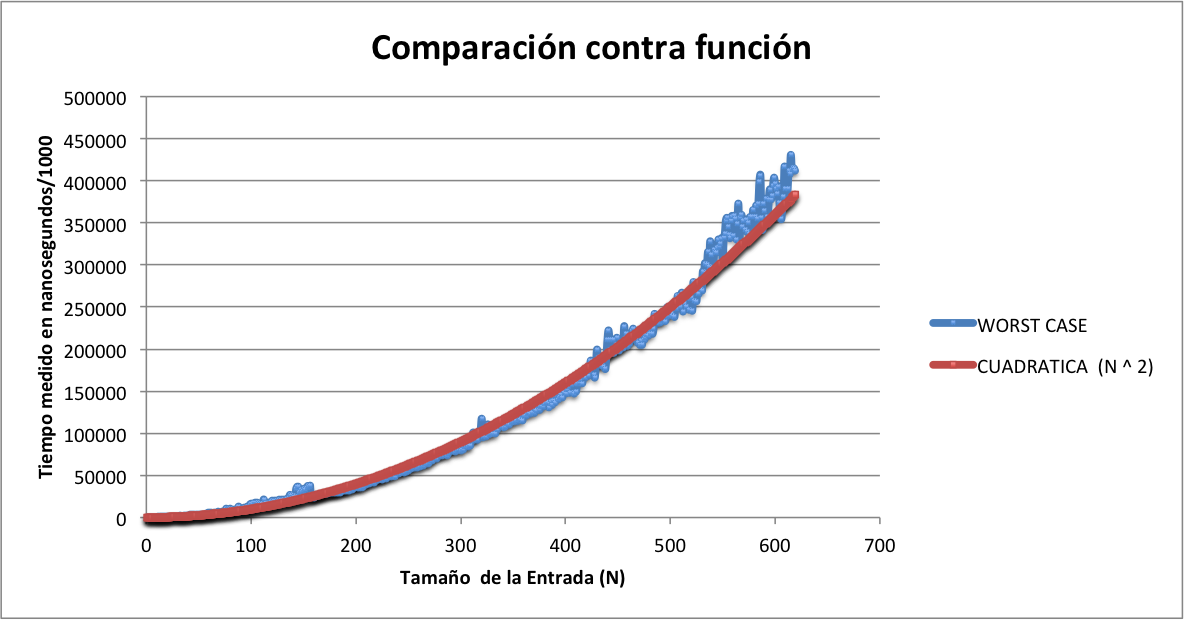
\includegraphics[width=120mm]{ej2_casos.png}
\centering
\caption{Peor caso en comparaci\'on con una funci\'on cuadr\'atica.}
\label{overflow3}
\end{figure}
Como mencionamos antes, el peor caso sucede cuando debemos recorrer todos los nodos. La cantidad de nodos viene dada por $N*L$. Para hacer los tests, decidimos utilizar edificios de forma cuadrada, es decir que la cantidad de pisos es igual a la longitud de cada piso. Para estos casos, tenemos que $L = N$. Y como se ve en el grafico, el peor caso se comporta muy similar a esta manera. 

\begin{figure}[h!]
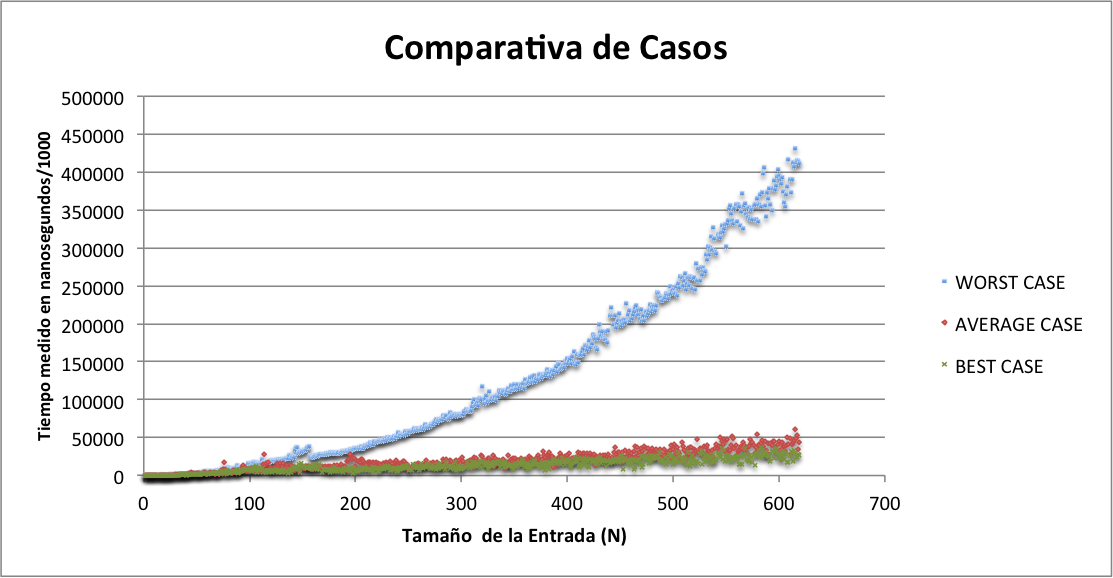
\includegraphics[width=120mm]{ej2_comp.png}
\centering
\caption{Comparaci\'on de los peores y mejores casos contra casos promedio.}
\label{overflow3}
\end{figure}
Como podemos apreciar en el grafico, el caso promedio se aleja muchisimo del peor caso ya que al general de manera pseudo-aleatoria las conexiones entre los portales, la probabilidad de tener que recorrerlos absolutamente todos ( $N*P+L$) es muy baja. Llamativamente, el caso promedio se asemeja al mejor caso. Creemos que la causa es que como un portal puede tener muchos vecinos, podemos encontrar el camino al final de manera mas rapida.

\subsubsection{Optimizado vs no optimizado}
Para mejorar el rendimiento del algoritmo se agrego una optimizacion donde al momento de encontrar el nodo buscado finalizara, a continuacion se haran algunas pruebas sobre el beneficio que brinda dicha optimizacion en los casos vistos en la secci\'on $2.4$.
\\
Primero veamos un poco el algoritmo:

\begin{lstlisting}
solve(Nodo nodo, Nodo nodo2, int i) 
	cola <- new LinkedList<Nodo>()
	cola.addFirst(nodo)
	nodo.setVisitado()
	WHILE ! cola.isEmpty()
        Nodo actual;
        actual = cola.pop()
        List<Nodo> vecinos = actual.getVecinos();		
        FOREACH vecinos AS vecino
            IF !vecino.getVisitado()
                vecino.setVisitado()
                vecino.setLongitud(actual.getLongitud()+1)
			cola.push(vecino)
	        ENDIF
     	ENDFOR
    ENDWHILE
DEVOLVER nodo2.getLongitud()
\end{lstlisting}

Por como esta dado simplemente chequeara todos los nodos y, al terminar, quedara en $nodo2$ la longitud minima, a continuacion se considerara el siguiente codigo:

\begin{lstlisting}
solve(Nodo nodo, Nodo nodo2, int i) 
	cola <- new LinkedList<Nodo>()
	cola.addFirst(nodo)
	nodo.setVisitado()
	encontrado <- false
	WHILE !cola.isEmpty() AND !encontrado
        Nodo actual;
        actual = cola.pop()
        List<Nodo> vecinos = actual.getVecinos();		
        FOR i<-0 WHILE i<vecinos.size() AND !encontrado STEP i++ 
            vecino <- vecinos.obtener(i)
            IF !vecino.getVisitado()
                vecino.setVisitado()
                vecino.setLongitud(actual.getLongitud()+1)
                IF actual.getId() == nodo2.getId()
                    encontrado <- true
                ENDIF
            cola.push(vecino)
            ENDIF
     	ENDFOR
    ENDWHILE
DEVOLVER nodo2.getLongitud()
\end{lstlisting}

La variable encontrado sera colocada en true al momento de toparse con el nodo que era buscado, a primera vista esto deberia mejorar la performance del algoritmo, para ello se hara un analisis de cada caso: \\\\

\begin{centering}
Peor Caso \\
\end{centering}

\begin{figure}[h!]
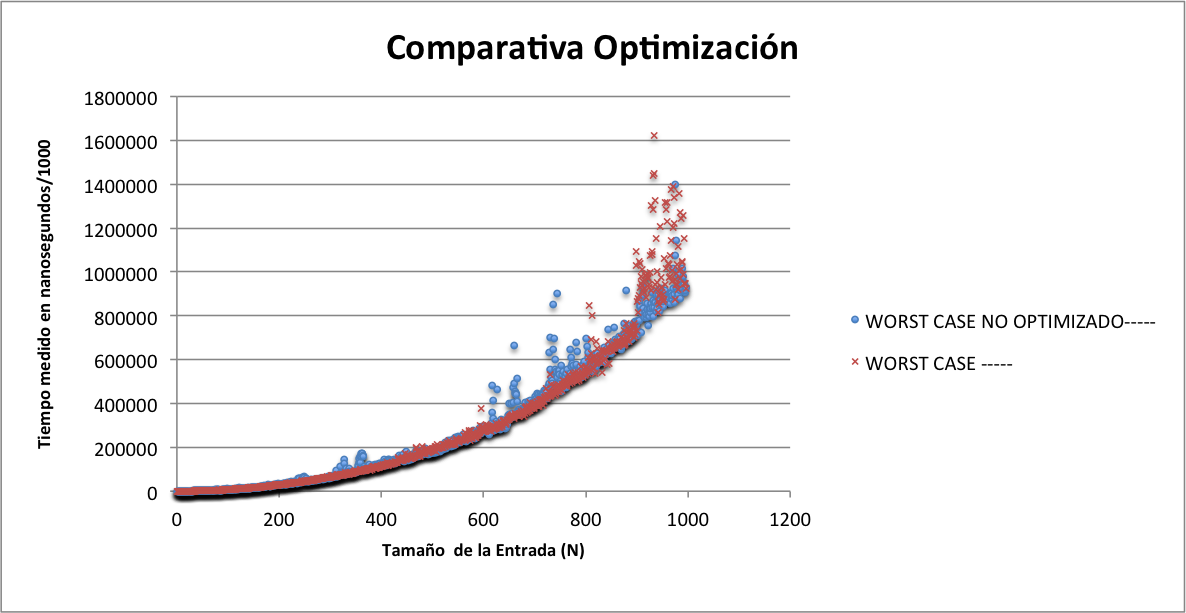
\includegraphics[width=140mm]{ej2-comp-tp2.png}
\centering
\caption{Comparacion peores casos}
\label{overflow3}
\end{figure}

En la imagen se puede observar que no hay una gran diferencia entre los dos algoritmos, esto se debe a que en el peor caso solo habra una conexion con el ultimo piso y esta estara al final del recorrido, por lo que cualquiera de los dos algoritmos debera recorrer todo el grafo hasta llegar al nodo buscado. Incluso podemos decir que el algoritmo optimizado puede tardar un poco ya que posee $3$ chequeos intermedios sobre la variable $encontrado$, que si bien no es un gran cambio afecta un poco.\\\\

\pagebreak

\begin{centering}
Mejor Caso \\
\end{centering}

\begin{figure}[h!]
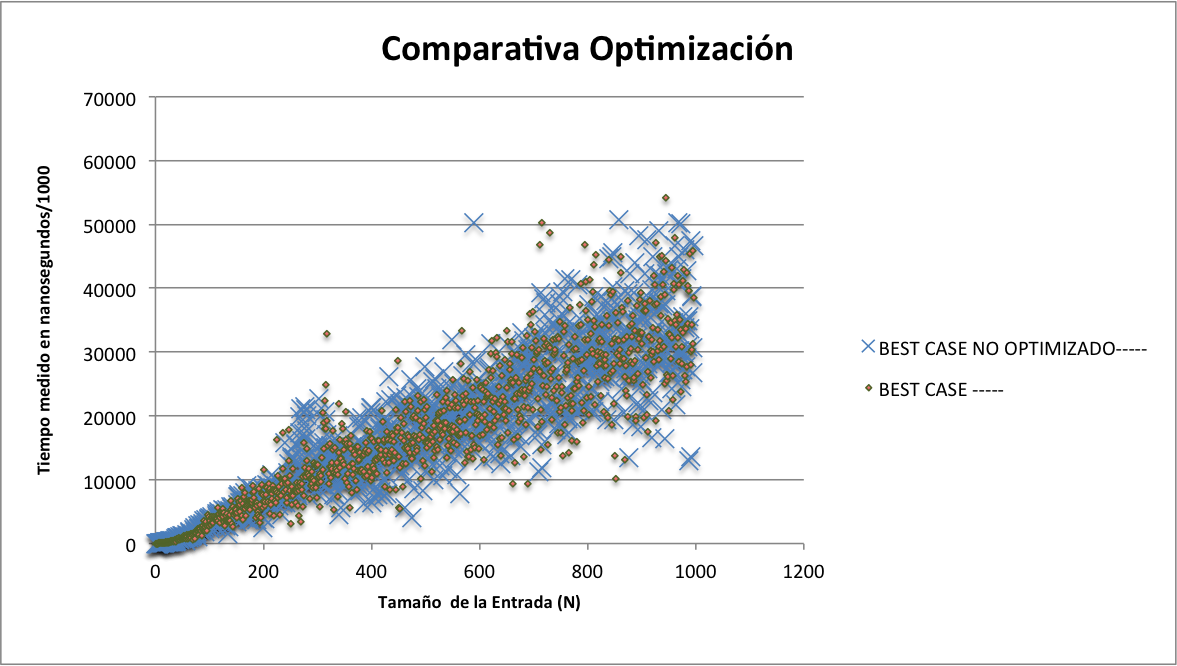
\includegraphics[width=140mm]{ej2-comp2-tp2.png}
\centering
\caption{Comparacion mejores casos}
\label{overflow3}
\end{figure}

En el mejor caso se construyo el grafo de manera que hubiera un portal apenas comienza el piso $0$ que conecte con el final del ultimo piso. Se espero que el rendimiento del algoritmo optimizado fuera superior al otro pero en el grafico se puede observar que no. 

\begin{figure}[h!]
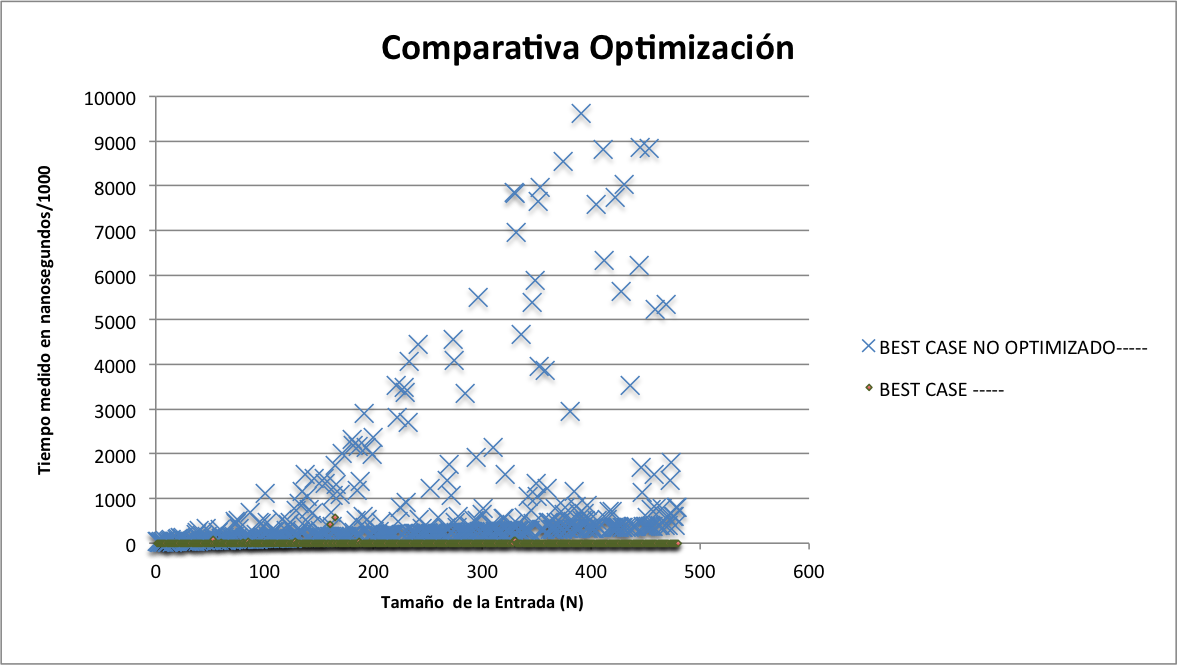
\includegraphics[width=140mm]{ej2-compesp-tp2.png}
\centering
\caption{Comparacion cantidad de iteraciones mejores casos}
\label{overflow3}
\end{figure}

Haciendo mas pruebas se pudo ver que el algoritmo optimizado casi siempre hizo $4$ iteraciones (ya que al tener portales lanzados aleatoriamente puede haberlo enviado a otro lugar) antes de terminar mientras que el otro tuvo cantidad variable y creciente, lo que contradice el primer grafico. La hipotesis es que hay algun costo externo que no pudo ser observado en la experimentacion. Pero teoricamente y por la prueba de iteraciones maximas podemos decir que el algoritmo optimizado para este caso es mucho mas efectivo que el otro, teniendo un costo de $4$ iteraciones constantemente.\\\\

\pagebreak

\begin{centering}
Caso General \\
\end{centering}

\begin{figure}[h!]

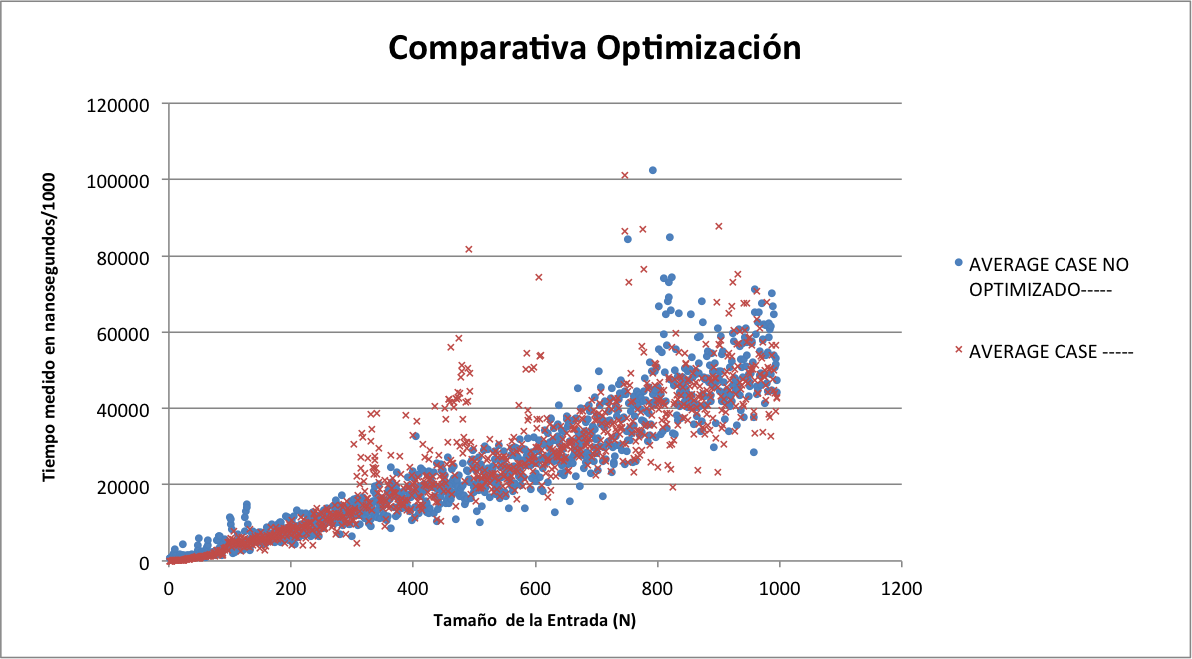
\includegraphics[width=140mm]{ej2-comp1-tp2.png}
\centering
\caption{Comparacion casos generales}
\label{overflow3}
\end{figure}

En el caso general el algoritmo optimizado tuvo un poco mas de rendimiento que el otro, se puede observar en el grafico que su curva tiene una pendiente menos eleveda que el no optimizado, como en el caso general no sabemos cual es el camino general, el primer algoritmo tiende a ser un poco mejor.


\pagebreak
Luego decidimos comparar el mejor y peor caso del algoritmo, y analizamos los tiempos teniendo en cuenta la creaci\'on del grafo o no. En la siguiente imagen se observa la gran diferencia de tiempos y esto es debido al gran costo de incializaci\'on de estructuras.
\begin{figure}[h!]
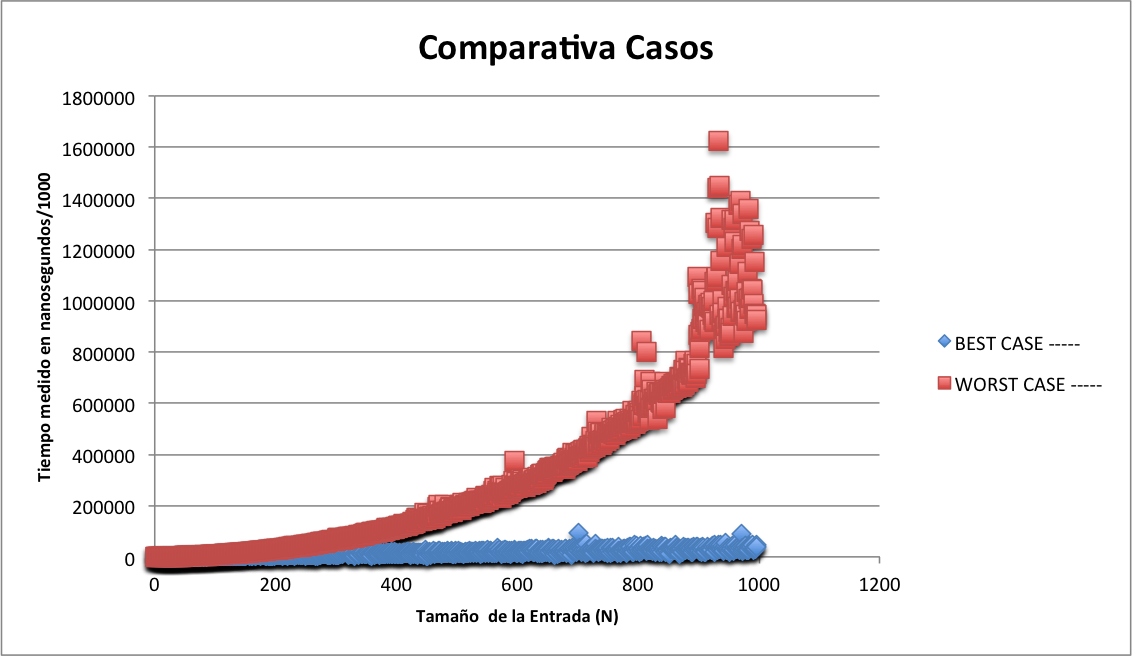
\includegraphics[width=140mm]{ej2-compcasos-tp2.png}
\centering
\caption{Comparacion Best Vs Worst}
\label{overflow3}
\end{figure}

\pagebreak


\pagebreak
\section{Ejercicio 3}

\subsection{Problema: Perdidos en los Pasillos}
El Pabell\'on 0+infinito, nuevamente remodelado, ahora tiene un disen\~o basado en un conjunto de M pasillos de distintas longitudes con intersecciones en donde se unen dos o m\'as pasillos. Es as\'i que puede modelarse como un grafo con pesos en los ejes, donde cada eje es un pasillo (de peso igual a la longitud del pasillo), y cada v\'ertices es una intersecci\'on o un extremo donde termina un pasillo sin unirse con ningu\'n otro. El decano junto con el director del Departamento de Computaci\'on, est\'an preocupados porque talvez existen ciclos en dicho grafo, lo que podr\'ia perjudicar a los alumnos al hacer que se pierdan buscando las aulas. Por tal motivo el decano decidi\'o clausurar los pasillos que sea necesario de manera tal que no queden ciclos en el grafo que representa al pabell\'on. El problema es que cuanto m\'as largo es un pasillo, m\'as costoso es clausurarlo. Disen\~ar un algoritmo de complejidad O(M log M ) para calcular la m\'inima suma posible de las longitudes de los pasillos que deber\'ian ser clausurados (eventualmente ninguno) para que no existan ciclos formados por tres o m\'as pasillos en el grafo que representa al pabell\'on. Se asegura que en toda instancia del problema el grafo que representa al pabell\'on es conexo.

\subsubsection{Explicacion del Problema}

    En este problema se tiene un edificio con pisos de longitud variable y portales que comunican pisos entre si. Por enunciado, este se puede representar como un grafo con pesos en sus ejes.
    
        %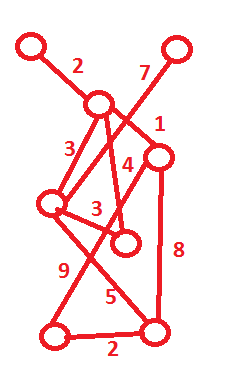
\includegraphics[scale=0.9]{imagenes/ejemploej3.png}\endl
        \begin{center}
\tikzset{main node/.style={circle,fill=white!20,draw,minimum size=0.75cm,inner sep=0pt},}
\begin{tikzpicture}
    
        \node[main node] (1) {1};
        \node[main node] (2) [right = 3.5cm of 1]  {$2$};
        \node[main node] (3) [above = 1.5cm of 1]  {$3$};
        \node[main node] (4) [right = 1.9cm of 3]  {$4$};
        
        \node[main node] (5) [above = 3.5cm of 2]  {$5$};
        \node[main node] (6) [left  = 1.8cm of 5]  {$6$};
        \node[main node] (7) [above = 2.5cm of 3]  {$7$};
        \node[main node] (8) [right = 3.5cm of 7]  {$8$};
    
        \path[draw,thick]
        (1) edge node {$2$} (2)
        (2) edge node {$5$} (3)
        (2) edge node {$8$} (5)
        (3) edge node {$3$} (4)
        (3) edge node {$7$} (8)
        (3) edge node {$3$} (6)
        (4) edge node {$4$} (6)
        (5) edge node {$1$} (6)
        (5) edge node {$9$} (1)
        (6) edge node {$2$} (7)
        (7) edge node {$2$} (8)
        ;
    
\end{tikzpicture}

    \\Ejemplo de grafo que representa el problema
\end{center}
        
    Lo que se quiere es eliminar (en el que caso de hubiera un ciclo) la menor cantidad de metros de pasillo posible (minima cantidad de peso total del ciclo) de manera tal que el grafo siga siendo conexo.
    
     %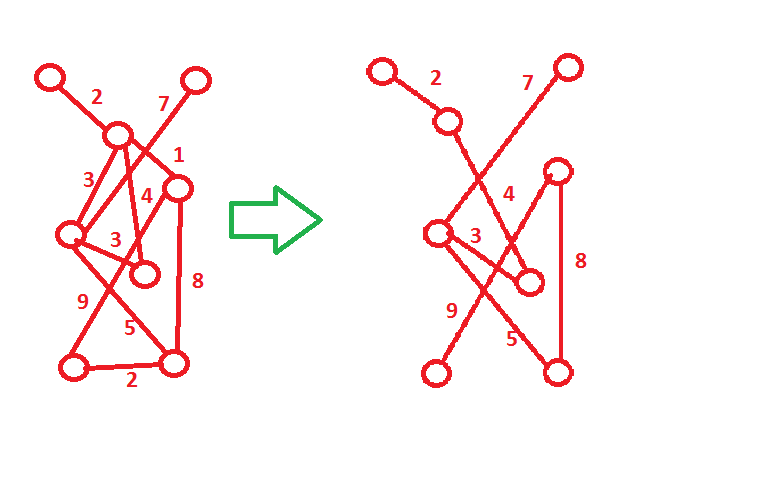
\includegraphics[scale=0.9]{imagenes/arbolgenmax.png}\endl
     \tikzset{main node/.style={circle,fill=white!20,draw,minimum size=0.75cm,inner sep=0pt},}
\begin{tikzpicture}
    \node[main node] (1) {1};
    \node[main node] (2) [right = 3.5cm of 1]  {$2$};
    \node[main node] (3) [above = 1.5cm of 1]  {$3$};
    \node[main node] (4) [right = 1.9cm of 3]  {$4$};
    
    \node[main node] (5) [above = 3.5cm of 2]  {$5$};
    \node[main node] (6) [left  = 1.8cm of 5]  {$6$};
    \node[main node] (7) [above = 2.5cm of 3]  {$7$};
    \node[main node] (8) [right = 3.5cm of 7]  {$8$};

    \path[draw,thick]
    (1) edge node {$2$} (2)
    (2) edge node {$5$} (3)
    (2) edge node {$8$} (5)
    (3) edge node {$3$} (4)
    (3) edge node {$7$} (8)
    (3) edge node {$3$} (6)
    (4) edge node {$4$} (6)
    (5) edge node {$1$} (6)
    (5) edge node {$9$} (1)
    (6) edge node {$2$} (7)
    (7) edge node {$2$} (8)
    ;
    
    \begin{scope}[xshift=7cm]
    \node[main node] (1) {1};
    \node[main node] (2) [right = 3.5cm of 1]  {$2$};
    \node[main node] (3) [above = 1.5cm of 1]  {$3$};
    \node[main node] (4) [right = 1.9cm of 3]  {$4$};
    
    \node[main node] (5) [above = 3.5cm of 2]  {$5$};
    \node[main node] (6) [left  = 1.8cm of 5]  {$6$};
    \node[main node] (7) [above = 2.5cm of 3]  {$7$};
    \node[main node] (8) [right = 3.5cm of 7]  {$8$};

    \path[draw,thick]
    (2) edge node {$5$} (3)
    (2) edge node {$8$} (5)
    (3) edge node {$3$} (4)
    (3) edge node {$7$} (8)
    (4) edge node {$4$} (6)
    (5) edge node {$9$} (1)
    (6) edge node {$2$} (7)
    ;
    \end{scope}
\end{tikzpicture}

\begin{center}
    \\Grafo donde fueron eliminados los ejes menos pesados de los ciclos
\end{center}
     
    En el ejemplo se tomaron los pasillos de menor tamaño dando de baja tan solo 6 metros\endl
        
\subsubsection{Explicaci\'on del Desarrollo}
    Para resolver el problema se planteo eliminar el eje de menor peso en cada ciclo para asi eliminar la menor cantidad de metros posible de manera que el grafo siga siendo conexo. 
    
    Analizandolo podemos ver que el resultado de eliminar estos ejes resulta en un arbol, el cual por haber eliminado los ejes de menor peso resulta ser el arbol generador maximo. Dicho esto el problema queda reducido a generar el arbol generador maximo del grafo, recordemos que la complejidad debe quedar acotada por $O(M * log M)$. Para generar el arbol se recurrio al algoritmo de kruscal, si bien este genera el arbol generador minimo, si se multiplican todos los pesos por $-1$ el arbol generador minimo sera el maximo del grafo (esto se analizara en detalle en la seccion $3.3$).\\
    
    Si bien kruscal genera el el AGM que se busca no cumple con la complejidad pedida ya que buscar el eje de menor peso y agregarlo a los revizados no tiene (por lo pronto) tiempo constante, para esto se recurrio a $Union Find$ con las huristicas $path compression$ y $link-by-rank$ (Ver seccion $3.3$).
    
    A continuaci\'on vemos el funcionamiento del Algoritmo de Kruskal.
    \begin{center}
\tikzset{main node/.style={circle,fill=white!20,draw,minimum size=0.70cm,inner sep=0pt},}
\begin{tikzpicture}
        \node[main node] (1) {0};
        \node[main node] (2) [right = 3.5cm of 1]  {1};
        \node[main node] (3) [above = 1.5cm of 1]  {2};
        \node[main node] (4) [right = 1.9cm of 3]  {3};
        \node[main node] (5) [above = 3.5cm of 2]  {4};
        \node[main node] (6) [left  = 1.8cm of 5]  {5};
    
        \path[draw,thick]
        (1) edge node {$2$} (2)
        (2) edge node {$5$} (3)
        (2) edge node {$8$} (5)
        (3) edge node {$3$} (4)
        (3) edge node {$3$} (6)
        (4) edge node {$4$} (6)
        (5) edge node {$1$} (6)
        (5) edge node {$9$} (1)
        ;
        
        \node[draw] at (2,-1) {Grafo original};
        
        \begin{scope}[xshift=6cm]
            \node[main node] (1) {0};
            \node[main node] (2) [right = 3.5cm of 1]  {1};
            \node[main node] (3) [above = 1.5cm of 1]  {2};
            \node[main node] (4) [right = 1.9cm of 3]  {3};
            
            \node[main node] (5) [above = 3.5cm of 2]  {4};
            \node[main node] (6) [left  = 1.8cm of 5]  {5};
        
            \path[draw,thick]
            (5) edge[red] node {$1$} (6)
            ;
            \node[draw] at (2,-1) {Agrega 1};    
        \end{scope}

        \begin{scope}[yshift=-7cm]
            \node[main node] (1) {0};
            \node[main node] (2) [right = 3.5cm of 1]  {1};
            \node[main node] (3) [above = 1.5cm of 1]  {2};
            \node[main node] (4) [right = 1.9cm of 3]  {3};
            
            \node[main node] (5) [above = 3.5cm of 2]  {4};
            \node[main node] (6) [left  = 1.8cm of 5]  {5};
        
            \path[draw,thick]
            (1) edge[red] node {$2$} (2)
            (5) edge node {$1$} (6)
            ;
            \node[draw] at (2,-1) {Agrega 2};    
            
        \end{scope}
        
        \begin{scope}[yshift=-7cm,xshift=6cm]
            \node[main node] (1) {0};
            \node[main node] (2) [right = 3.5cm of 1]  {1};
            \node[main node] (3) [above = 1.5cm of 1]  {2};
            \node[main node] (4) [right = 1.9cm of 3]  {3};
            
            \node[main node] (5) [above = 3.5cm of 2]  {4};
            \node[main node] (6) [left  = 1.8cm of 5]  {5};
        
            \path[draw,thick]
            (1) edge node {$2$} (2)
            (5) edge node {$1$} (6)
            (3) edge[red] node {$3$} (6)
            ;
            \node[draw] at (2,-1) {Agrega 3};    
        \end{scope}
        
        \begin{scope}[yshift=-14cm]
            \node[main node] (1) {0};
            \node[main node] (2) [right = 3.5cm of 1]  {1};
            \node[main node] (3) [above = 1.5cm of 1]  {2};
            \node[main node] (4) [right = 1.9cm of 3]  {3};
            
            \node[main node] (5) [above = 3.5cm of 2]  {4};
            \node[main node] (6) [left  = 1.8cm of 5]  {5};
        
            \path[draw,thick]
            (1) edge node {$2$} (2)
            (5) edge node {$1$} (6)
            (3) edge node {$3$} (6)
            (3) edge[red] node {$3$} (4)
            ;
            \node[draw] at (2,-1) {agrega 3};    
        \end{scope}
        
        \begin{scope}[yshift=-14cm, xshift=6cm]
            \node[main node] (1) {0};
            \node[main node] (2) [right = 3.5cm of 1]  {1};
            \node[main node] (3) [above = 1.5cm of 1]  {2};
            \node[main node] (4) [right = 1.9cm of 3]  {3};
            
            \node[main node] (5) [above = 3.5cm of 2]  {4};
            \node[main node] (6) [left  = 1.8cm of 5]  {5};
        
            \path[draw,thick]
            (1) edge node {$2$} (2)
            (5) edge node {$1$} (6)
            (3) edge node {$3$} (6)
            (3) edge node {$3$} (4)
            (4) edge[blue] node {$4$} (6)
            ;
            \node[draw] at (2,-1) {Al intentar agregar 4 se forma un circuito};    
        \end{scope}
\end{tikzpicture}

\newpage
\begin{tikzpicture}
    \begin{scope}[yshift=-21cm]
        \node[main node] (1) {0};
        \node[main node] (2) [right = 3.5cm of 1]  {1};
        \node[main node] (3) [above = 1.5cm of 1]  {2};
        \node[main node] (4) [right = 1.9cm of 3]  {3};
        
        \node[main node] (5) [above = 3.5cm of 2]  {4};
        \node[main node] (6) [left  = 1.8cm of 5]  {5};
    
        \path[draw,thick]
        (1) edge node {$2$} (2)
        (5) edge node {$1$} (6)
        (3) edge node {$3$} (6)
        (3) edge node {$3$} (4)
        (2) edge[red] node {$5$} (3)
        ;
        \node[draw] at (2,-1) {Al agregar 5 se termina de formar el arbol};    
    \end{scope}
\end{tikzpicture}

    \\algoritmo de kruskal para arbol generador minimo salteando los pasos finales donde solo saltea ejes.
\end{center}

\subsection{Justificaci\'on y Complejidad}

\begin{lstlisting}
grafo <- new Grafo();        // O(1)
FOREACH pasillos as pasillo  // O(M)
    grafo.addVertice(pasillo.getExtremo1(), pasillo.getExtremo2(),
    pasillo.getLongitud());
ENDFOREACH
union <- new UnionFind(grafo.getVertices().size() + 1); // O(M)
\end{lstlisting}


Veamos el costo de la funcion addVertice con mas detalle 

\begin{lstlisting}
addVertice(int nodo1, int nodo2, int peso ) 
	vertice <- new Vertice(nodo1, nodo2, -peso); // O(1)
	vertice.setId(idVertices); // O(1)
	idVertices++;	// O(1)
	vertices.add(vertice); // O(1)
	this.peso += peso; // O(1)
	}
\end{lstlisting}
Costo final de la funci\'on addVertice $\bigO(1)$, por lo tanto el costo de la creaci\'on del grafo es $\bigO(M)$

\begin{lstlisting}
vertices <- grafo.getSortedVertices(); // O(M * log(M))
i = 0;
peso = 0;
WHILE i < vertices.size()
	IF union.find((Integer)vertices.get(i).getNodo1()) != union.find((Integer)vertices.get(i).getNodo2())
	THEN   
	union.union((Integer)vertices.get(i).getNodo1(),
	(Integer) vertices.get(i).getNodo2());
	peso += vertices.get(i).getPeso();
	ENDIF
	i++;
		}
ENDWHILE
DEVOLVER -( ( grafo.getPeso()*-1 ) - peso;
\end{lstlisting}
\subsection{Correctitud}

    Primero observemos que los pesos del grafo $G$ fueron modificados por su peso multiplicado por $-1$ lo que da otro grafo $G'$, esto hace que todos los pesos queden negativos. luego se corre el algoritmo de kruskal sobre ese grafo, por lo visto en clase este nos dara el arbol generador minimo de $G'$ que por $Lema 3.1$ resulta ser el arbol generador maximo de $G$. \\
    
    Ahora veamos que el arbol generador maximo de $G$ resuelve el problema: Se necesita cerrar la menor cantidad de metros de pasillo tal que no queden ciclos entonces se debe sacar el eje de menor peso de cada ciclo, sea e el eje de meor peso de algun ciclo de $G$ entonces el arbol generador maximo tomara primero los ejes mas grandes del algun ciclo, dado que e es el menor de los ejes de algun ciclo al momento en el que es tomado ya fueron agregados $k$ ejes al arbol generador tal que $\forall k_i$ $p(k_i) >= p(e)$. si agrego $e$ al arbol se formara un ciclo ya que como $e$ tiene el menor peso del mismo sera tomado ultimo. A continuaion como $e$ genera un ciclo no es agregado al arbol $\rightarrow$ el eje que no es agregado al arbol generador maximo es el de peso minimo. \\
    
    Con esto queda probado que para todo ciclo del grafo $G$ los unicos ejes que seran removidos seran los de menor peso dentro de los ciclos.
    
    \subsubsection{Lema 3.1}
    Dado un grafo $G$ con pesos en sus ejes y dado $G'$ un grafo tal que $V(G) = V(G')$ y $\forall e \in E(G), e' \in E(G')$ $p(e) * -1 = p(e') \rightarrow$ el arbol generador minimo de $G$ es el arbol generador maximo de $G'$ \\
    
    Sea $H$ el peso del AGM en $G$, y sea $n$ la cantidad de sus vertices, como sabemos que es un arbol tiene $n -1$ ejes. Entonces sabemos que $H$= \displaystyle\sum_{k=1}^{N-1}   P(e_k).\\ \endl
           
    Tambien sabemos que, al contener a todos los vertices, independientemente del valor de sus ejes, tambien es un arbol generador en el grafo $g'$. Sea $T$ el peso de este arbol generador de $g'$
    Entonces $T =  \displaystyle\sum_{k=1}^{N-1}  P(e_k)*-1 $\\ \endl
    Y como la multiplicacion es distributiva, tenemos que $T =[  \displaystyle\sum_{k=1}^{N-1}  P(e_k) ]*-1$ \\
    Entonces tenemos que $T = H * -1$. Ahora sabemos, que H era un AGM por ende $\forall a$ arbol, $H \le$ Peso($a$). Reemplazando, tenemos que $\forall a$ arbol, $T/-1 \le Peso(a)$. Pero si paso el -1 para al pasar el -1 dividiendo, tenemos que dar vuelta la desigualdad, quedando que:
    $\forall a$ arbol, $T \ge$ Peso($a$). Osea Es Arbol Generador Maximo.
    
\subsection{Tests}
%INSERTAR DIBUJITO COMPARATIVO K5 LAS ARISTAS MAS PESADAS LAS DEL PENTAGONO Y CICLO DE 10 ARISTAS
    Para testear el mejor y peor caso decidimos comparar dos grafos que tengan la misma cantidad de aristas pero que difieran ampliamente en la cantidad de vertices. Describamoslo con un ejemplo: Tenemos por un lado el grafo $k5$, que tiene 10 aristas y por otro un ciclo simple de 11 vertices y 10 aristas. Lo que sucede es que el algoritmo de Kruskal corta al agregar la arista $n-1$(siendo n la cantidad de vertices) por ende en el segundo grafo, el algoritmo esta obligado a recorrer todas las aristas hasta conformar el AGM. Como vemos en la imagen, el algoritmo para el primer grafo, agregara todas las aristas que forman el pentagono y concluira sin haber revisado las aristas de la estrella.\\
    Ademas pudimos observar que dependiendo de los pesos de las aristas de $K_5$ podiamos tener un mejor y un peor caso, en el que por ejemplo generemos el Arbol generador solo mirando solo las aristas que son el AG en si mismo, o podiamos estar en el peor caso que seria un ciclo.\\ \\ 
    \\ \\ \\ \\ \\ 
    
    
    \begin{tabular}{ l c }
   \tikzset{main node/.style={circle,fill=white!20,draw,minimum size=0.5cm,inner sep=0pt},}
\usetikzlibrary{graphs,graphs.standard}

\begin{tikzpicture}

\def \n {10}
\def \radius {2cm}
\def \margin {8} % margin in angles, depends on the radius

\foreach \s in {1,...,10}
{
  \node[draw, circle] at ({360/\n * (\s - 1)}:\radius) {$\s$};
  \draw[->, >=latex, red] ({360/\n * (\s - 1)+\margin}:\radius)
    arc ({360/\n * (\s - 1)+\margin}:{360/\n * (\s)-\margin}:\radius);
}
  \node[draw, circle] at ({360/\n * (5 - 1)}:\radius) {$5$};
  \draw[->, >=latex] ({360/\n * (5 - 1)+\margin}:\radius)
    arc ({360/\n * (5 - 1)+\margin}:{360/\n * (5)-\margin}:\radius);

\end{tikzpicture} & \tikzset{main node/.style={circle,fill=white!20,draw,minimum size=0.5cm,inner sep=0pt},}
\usetikzlibrary{graphs,graphs.standard}

\begin{tikzpicture}
  \foreach \x in {1,...,5}{%
    \pgfmathparse{(\x-1)*360/5}
    \node[draw,circle,inner sep=0.25cm] (N-\x) at (\pgfmathresult:2.0cm) [thick] {};
  }
  \pgfmathparse{7*360/5}
  %\node[circle,red] (N-8) at (\pgfmathresult:5.4cm) {\ldots};
  
  \path (N-1) edge[ultra thin,-, red] (N-2);
  \path (N-2) edge[ultra thin,-, red] (N-3);
  \path (N-3) edge[ultra thin,-, red] (N-4);
  \path (N-4) edge[ultra thin,-, red] (N-5);
  
  \path (N-1) edge[ultra thin,-] (N-3);
  \path (N-1) edge[ultra thin,-] (N-4);
  \path (N-1) edge[ultra thin,-] (N-5);
  
  \path (N-2) edge[ultra thin,-] (N-4);
  \path (N-2) edge[ultra thin,-] (N-5);
  
  \path (N-3) edge[ultra thin,-] (N-5);
  
\end{tikzpicture} \\
\end{tabular}
    
    
    
\pagebreak
\subsubsection{Performance}
%actualizar grafico%
En esta secci\'on utilizaremos lo mencionado en los tests: Vamos a comparar que diferencia hay entre dos grafos que tienen la misma cantidad de aristas, difieran ampliamente en la cantidad de vertices y que ademas, las  $n-1$ aristas mas pesadas, sean las que efectivamente conforman nuestro AGM. Con esto ultimo logramos que el algoritmo de Kruskal corte mucho antes de tener que recorrer todas las aristas del grafo.
Esta idea la conceptualizamos en el siguiente gr\'afico, en el cu\'al se observa que la cantidad de aristas que revisa el algoritmo de Kruskal es mucho mayor para el grafo donde, a misma cantidad de aristas, menor cantidad de vertices.\\

\begin{figure}[h!]
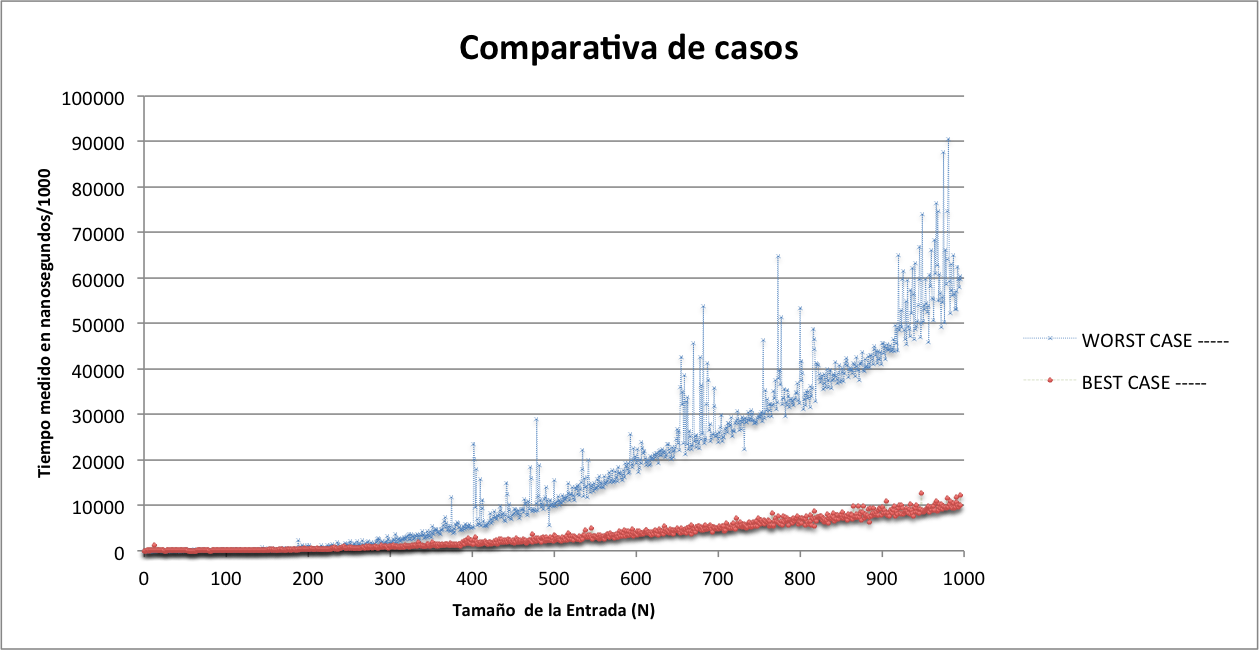
\includegraphics[width=140mm]{ej3-comp-tp2.png}
\centering
\caption{Tiempo de ejecuci\'on en funci\'on de la cantidad de aristas.}
\label{overflow3}
\end{figure}

\pagebreak
Luego decidimos ver que sucedia si no elegiamos las aristas del k5 para estar en un mejor caso y decidimos hacer que los pesos que se le asigaban fuesen random. En el siguiente grafico se observan cosas interesantes, como puede ser que hay dos o tres casos en el cual el random de pesos cayo en el mejor caso, pero tambien vemos que es muy particular ya que la mayoria de casos se mantienen con el crecimiento de la complejidad. 
\begin{figure}[h!]
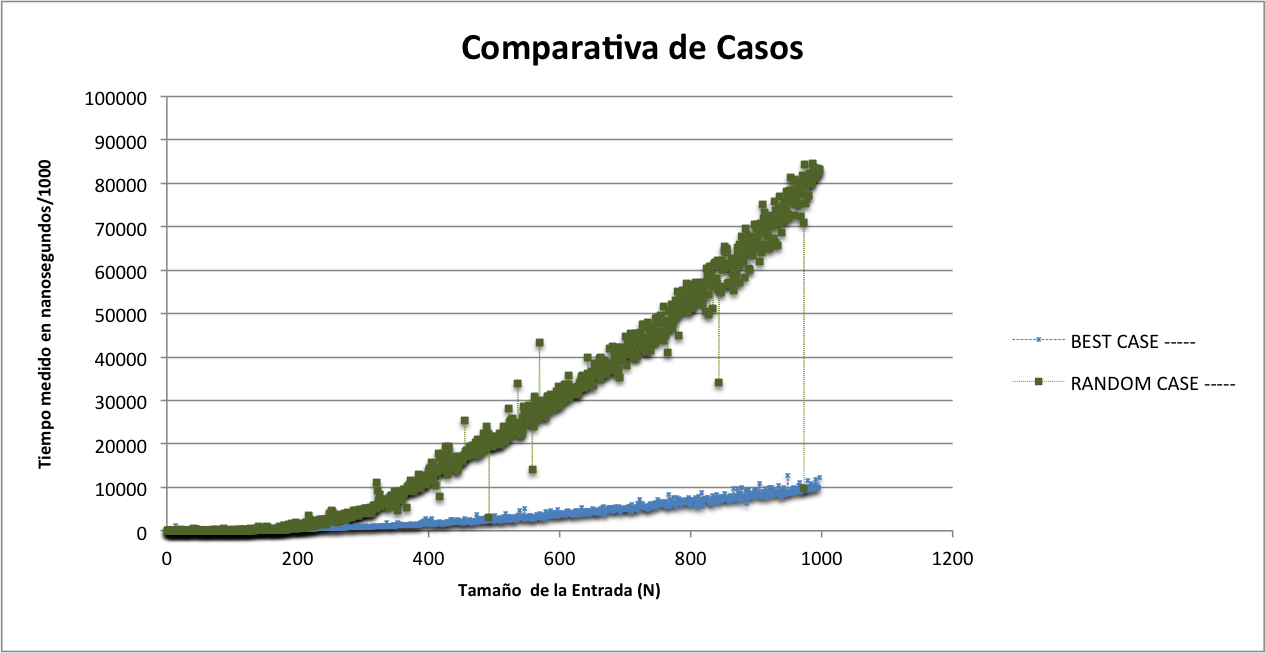
\includegraphics[width=140mm]{ej3-comp2-tp2.png}
\centering
\caption{Tiempo de ejecuci\'on en funci\'on de la cantidad de aristas.}
\label{overflow3}
\end{figure}

Hay tres picos en las medici\'ones del caso random, esto lo consideramos como ruido de la virtual machine de java en la que corrieron nuestros tests.


\pagebreak
\section{Apendice}
\subsection{Cambios en Reentrega}
    En estos ejercicio se:
\subsubsection{Ejercicio 1}
    -Mejoraron los casos de test y se rehicieron los graficos explicativos.\\
    -Se rehizo la Correctitud.\\
    -Se agregaron comentarios a la Justificaci\'on y Complejidad.
\subsubsection{Ejercicio 2}
    -Se amplio la explicacion y el desarrollo del problema\\
    -Se saco la demostracion de BFS por haber sido vista en clase\\
    -Se cambio la estructura para almacenar los nodos, ahora utilizamos una matriz.\\
    -Arreglo el an\'alisis de complejidad.\\
    -Se modifico el metodo $connect$ dentro de la clase $Grafo2$ para que tuviera en cuenta portales dentro de un mismo piso\\
    -Se agrego la posibilidad de solucionar el problema sin la optimizacion de cortar al encontrar el nodo buscado\\
    -Cambiaron los tests para experimentar $optimazacion vs no optimizacion$\\
\subsubsection{Ejercicio 3}
    -Se Amplio la explicacion y el desarrollo del problema\\
    -Se saco la demostracion de Kruscal por haber sido vista en clase\\
    -Se mejoraron los casos de test y se re hicieron los graficos explicativos.
    - Se agregaron euristicas al union find para mejorar su complejidad. (By Rank y Path Compresion).

\end{document}
